\documentclass[11pt,oneside]{scrartcl}
\usepackage[a4paper,total={6.5in, 9.0in}]{geometry}

\newcommand{\mchname}{Mat\'{u}\v{s} Chochl\'{i}k}
\newcommand{\mchmail}{chochlik@gmail.com}
\newcommand{\doctitle}{Static reflection}
\newcommand{\docsubtitle}{Rationale, design and evolution.}
\newcommand{\docnum}{P0385R1}
\newcommand{\docdate}{2016-10-13}

\usepackage[utf8]{inputenc}
\usepackage{url}
\usepackage[colorlinks=false,hidelinks]{hyperref}
\usepackage{parskip}
\usepackage[titletoc]{appendix}
\usepackage{siunitx}
\usepackage{dirtytalk}
\usepackage{color,soul}
\usepackage{enumitem}
\usepackage{cite}

\usepackage{listings}
\usepackage{minted}
\lstset{basicstyle=\footnotesize\ttfamily,breaklines=true}

\usepackage{fancyhdr}
\setlength{\headheight}{14pt}
\pagestyle{fancyplain}
\lhead{\fancyplain{}{\textbf{\docnum} -- \doctitle\\\scriptsize{\docsubtitle}}}
\rhead{}
\rfoot{\fancyplain{}{\thepage}}
\cfoot{}

\usepackage[pdftex]{graphicx}
\DeclareGraphicsExtensions{.pdf}
\usepackage{rotating}

\setcounter{tocdepth}{3} 

\title{\doctitle}
\subtitle{\docsubtitle}

\author{\mchname (\mchmail)}

\newcommand{\concept}[1]{{\em{#1}}}
\newcommand{\meta}[1]{\textbf{\em{Meta-#1}}}

\begin{document}

\begin{tabular}{r l}
Document number: & \docnum\\
Date: & \docdate\\
Project: & Programming Language C++ \\
Audience: & Reflection (SG7) / EWG \\
	Reply-to: & \mchname (\href{mailto:\mchmail}{\mchmail}), Axel Naumann (\href{mailto:axel@cern.ch}{axel@cern.ch}), David Sankel (\href{mailto:camior@gmail.com}{camior@gmail.comr})\\
\end{tabular}

\begin{center}
\vskip 2em
{\Huge \doctitle}\\
{\Large \docsubtitle}
\vskip 1em
{\em \mchname, Axel Naumann}
\vskip 2em
\end{center}

\paragraph{Abstract}

The aim of this paper is to provide the rationale behind the
design of the static reflection facility proposed in P0194,
to enumerate and describe its potential use-cases
and to keep a written record of its evolution. It also answers questions
frequently asked in regard to the proposal.

\tableofcontents

\section{Introduction}

This paper accompanies the P0194Rx papers which we want to keep brief, technical
and to the point and which will eventually result in the final wording to be
included into the standard if this proposal is accepted.

We are writing this paper with several goals in mind:

\begin{itemize}
\item To define and explain the reflection-related terminology.
\item To keep a written record of the rationale behind the design of the
proposed static reflection facility.
\item To keep the answers to the frequently asked questions about
the decisions we've made in this proposal in one place so that we can avoid
having to write them over and over from scratch in various discussions\footnote
{Also to help us remember what the answers were.}.
\item To enumerate and describe the use cases for the various features
which we included in the proposal.
\item To provide concrete examples of usage.
\item To discuss the possibilities of the evolution of reflection in the future.
\end{itemize}

The text of this paper includes several revised, updated and extended parts
from the previous papers: N3996, N4111, N4451, N4452 and previous revisions
of P0385.

There is also an experimental implementation of the P0194R2 proposal
described in greater detail in section~\ref{implementation}
and the {\em Mirror} reflection library built on top of the proposed
static reflection facility described in section~\ref{mirror-lib}.

\subsection{Terminology}

In order to avoid confusion about terminology, this section provides definitions
for several important terms used throughout the text of the paper and
explains what we mean when using them in the context of this paper.

\subsubsection{Base-level, meta-level}
\label{term-base-meta-level}

When speaking generally, the {\em meta-level} is some higher level of abstraction
conceptually describing a lower, {\em base-level} which is the primary subject
of our endeavors.

In the context of this paper the base-level is the structure of a C++ program.
The meta-level is an abstraction partially describing that structure,
mainly the declarations of the program.

\subsubsection{Metadata}
\label{term-metadata}

{\em Metadata} is generally a piece of data conceptually describing some other,
{\em primary} data.

In the context of this paper, metadata is data providing information
about the base-level structure of a program.

{\em Static metadata} is metadata which can be manipulated or reasoned
about at compile-time by the compiler.

The metadata itself has its own structure.
For example metadata describing the base-level declaration of a class 
from a C++ program includes;
\begin{itemize}
\item the name of the class,
\item its scope,
\item list of its base classes,
\item list of data members,
\item list of nested types like type aliases, classes and enumerations,
\item the class key specifier, the access specifier,
\item source location information,
\item etc.
\end{itemize}

\subsubsection{Metaprogramming}

{\em Metaprogramming} is a kind of programming with the ability to treat and
manipulate other programs as data, so both the input and the output of
a metaprogram is usually a program. The language in which metaprograms
are written is called the {\em metalanguage} and it can be a different or the
same language as the one used to write the primary program.

C++ metaprogramming can be done both in an external language\footnote{For example a
C++ code generator written in Python or Bash.}, in a C++ compiler plug-in,
or in C++ itself. 

In C++ metaprogramming usually takes the form of an external
{\em source code generator}\footnote{Like Qt's MOC.}, or the form
of {\em preprocessor}, {\em template} or {\em constexpr} metaprogramming.

With template metaprogramming we use C++'s type system
as a standalone functional programming language \say{interpreted} by a C++
compiler, with \say{variables} being
represented by types (or compile-time constants),
\say{data structures} by instantiations of templates,
\say{subroutines} by class templates or template aliases, and
algorithms or \say{programs} by compositions of the above.

Unless stated otherwise when we say \say{metaprogramming} in the following text,
we mean template metaprogramming\footnote{Although we envision that
a constexpr-metaprogramming interface will also be added later in the future.}.

\subsubsection{Reflection}

In the context of computer science,
the term {\em reflection} refers to the ability of a program to examine
and possibly modify its own structure and/or behavior.

When combined with metaprogramming, this can include modification of the existing
or the definition of new data structures, doing changes to algorithms or changing the way
a program code is interpreted\footnote{Mostly in interpreted languages.}.

For the purpose of this paper -- {\em reflection is the process of obtaining
metadata}.

In the future the meaning can be expanded to include modification of the program
in ways exceeding the capabilities of current template
metaprogramming\footnote{For example generating new class data members.}.

\subsubsection{First-class object, second-class object}
\label{term-first-class}

First-class objects are also known as first-class {\em citizens}, {\em types},
{\em entities} or {\em values}.
In the context of programming language design they describe an entity that satisfies
the following:

\begin{itemize}
	\item{Can be stored in a named variable or a data structure.}
	\item{Can be passed as an argument to a subroutine.}
	\item{Can be returned as a result of a subroutine.}
	\item{Has an intrinsic identity making the entity unique and distinguishable.}
\end{itemize}

Since this paper deals with compile-time static reflection and its use
in compile-time metaprogramming, we will be talking about first- or second-class
citizens in this regard. 
For the purpose of this paper a first-class object is something that
we can distinguish and reason about at compile-time and what can be passed around
as \say{data} in metaprograms -- something that can be a template parameter.

This means that a type, a template instance or a compile-time integral constant
is for our purposes a first-class object:

\begin{minted}{cpp}
// compile-time "values"
struct value_a { };
struct value_b { };

// a compile-time "subroutine"
template <typename Param>
struct identity
{
	using result = Param;
};

// "values" are equality comparable and they are distinguishable
assert(!std::is_same_v<value_a, value_b>);
// and can be used for overloading
assert(!std::is_same_v<identity<value_a>, identity<value_b>>);

// they can be stored in named "variables" ...
using x = value_a;

// ... while maintaining their identity
assert(std::is_same_v<value_a, x>);

// they can be passed as parameters to subroutines
identity<value_a>;
identity<value_b>;

// they can be returned from subroutines
using y = identity<value_a>::result;
using z = identity<value_b>::result;

// ... while still maintaining their identity
assert(std::is_same_v<value_a, y>);
assert(std::is_same_v<value_b, z>);
// and still being distinguishable
assert(!std::is_same_v<y, z>);
\end{minted}


On the other hand a namespace, a type alias or a template parameter do not have
some or any of these properties.

\begin{minted}{cpp}
// other entities
namespace std { }
namespace foo = std;
using bar = unsigned;
using baz = unsigned;

template <typename Param>
struct identity
{
	using result = Param;
};

// they are not distinguishable
std::is_same_v<bar, baz>;
// and cannot be used for overloading
std::is_same_v<identity<bar>, identity<baz>>;

// they are not even comparable
std::is_same_v<std, foo>;

// they cannot be passed as arguments to subroutines
identity<std>;
identity<foo>;

// nor returned as a result
namespace y = identity<foo>::result;

// those which can be returned ...
using z = identity<bar>::result;
// ... do not maintain their unique identity
std::is_same_v<z, baz>;
\end{minted}

From the above follows, that a {\em second-class object} is everything else that
is not a first-class object, for example a namespace or a typedef.

\subsubsection{Reification}
\label{term-reification}

Generally speaking {\em reification} or \say{thingification}\footnote{From latin
\say{rei}, the dative form of \say{res} -- a thing.}, is making something
real, bringing it into being as an entity with its own identity,
or making something concrete.

In regard to programming languages, reification is often defined as making
an entity in the language a first-class object. So in the context of C++ template
metaprogramming a type is reified, but a namespace or a specifier is not.


\section{Revision history}

\subsection{P0385R0}

The initial revision of the design paper accompanying the P0194 papers.

\subsection{P0385R1}

This revision brought the following updates reflecting
the changes made in the P0194R2 paper.

\begin{itemize}
\item Based on the feedback from Oulu, the specification of typedef and
type alias reflection has been simplified. We no longer require reflection
to be aware of the whole chain of type aliases especially not in the context
of templates, each type alias only references the underlying type with unique
identity at the base level.
\item Unlike in the previous revision it is now possible to create variables
with {\em metaobject} types.
\item Section~\ref{fac-for-each} describing the \verb@for_each@ function
planned to be included in future revisions has been revised.
\item The {\em reverse reflection operator} has been renamed to \verb@unreflexpr@.
\item The {\em identifier-generating operator} has been renamed to \verb@idreflexpr@.
\item The mechanism for enumerating public-only vs. all (including non-public ones)
class members has been changed. Now the \say{basic} operations like
\verb@get_data_members@, \verb@get_member_types@, etc.
return all members, and the \verb@get_public_data_members@,
\verb@get_public_member_types@, return only the public class members.
\item All examples have been revised and extended according to the changes listed above.
\item New examples have been added to section~\ref{design-prefs} describing
the design considerations.
\item A description of the implementation has been added (section~\ref{implementation}).
\item A brief introduction to the {\em Mirror reflection utilities} has been added
(section~\ref{mirror-lib}).
\end{itemize}

\subsection{P0385R2 -- current revision}

We have made several big changes in revision R3 of the P0194 paper:

\begin{itemize}
\item We introduced the \verb@$@ character to the basic source character set
	as a prefix for all reflection-related operators -- both the primary
	reflection operator which is already part of the wording and for
	any which may be added in the future.
\item The reflection-related operators have been renamed
	\begin{itemize}
	\item from \verb@reflexpr@ to \verb@$reflect@,
	\item from \verb@unreflexpr@ to \verb@$unreflect@ and
	\item from \verb@idreflexpr@ to \verb@$identifier@.
	\end{itemize}
\item The reflection-related namespace has been renamed from \verb@std::meta@
	to \verb@std::reflect@ in order to avoid confusion and conflicts with
	any potential metaprogramming library which could be added in the future.
\item The reflection-related header file has been renamed from \verb@<reflexpr>@
	to \verb@<reflect>@.
\item Direct reflection of specifiers (previously \verb@reflexpr(public)@)
	and metaobjects reflecting specifiers (conforming to the \verb@Specifier@
	concept) have been removed temporarily and their functionality has been
	partially replaced with boolean traits.
\item The metaobject concept hierarchy has been slightly changed; in addition
	to the \verb@Specifier@, the \verb@TagType@ concept has
	also been removed, its operations were taken over by \verb@Enum@
	and \verb@Record@ concepts. The \verb@Reversible@ concept has also
	been removed for the time being.
\item The order of template parameters for \verb@MetaSequence@ operations has
	been matched to similar operations of \verb@std::tuple@.
\item The suffix \verb@_m@ was reverted back to \verb@_t@ for all
	metaobject-returning operations.
\end{itemize}

In this revision of P0385 we made the following changes:

\begin{itemize}
\item Some of the use-cases were removed for the sake of brevity, please see
	the previous revisions of this paper.
\item The examples have been updated to match the wording from P0194R3.
\end{itemize}


\section{Motivation}

Generic programming and metaprogramming supported by reflection can be valuable
tools in the implementation of an extensive range of various use cases or
programming patterns, including but not limited to:

\begin{itemize}

\item serialization or conversion of data from the native C++ representation
into a standard or custom, text-based or binary format like XML, JSON, XDR, ASN1,
etc.,

\item (re-)construction of instances of both \say{atomic} and structured types
from external data representations, like those listed above, or
from the data stored in a relational database, or from data entered by
a user through a user interface, or queried through a web service API,

\item automated implementation of comparison operations or hash functions
for structured types,

\item automated generation of user interface elements,

\item automatic generation of a relational schema from the application
object model and object-relational mapping (ORM),

\item support for scripting or implementation of input data parsers,

\item support for remote procedure calls (RPC) / remote method invocation (RMI),

\item inspection and manipulation of existing objects via a user interface
or a web service,

\item visualization of objects or structured data and their relationships,

\item automatic or semi-automatic implementation of certain software design
patterns, for example the factory pattern,

\item implementation of cross-cutting aspects like debugging, logging, profiling,
access control, etc.,

\item implementation of source code generators.

\end{itemize}

Some of the use cases listed above are described in more detail in section
\ref{use-cases-examples}.

There are several approaches to the implementation of the mentioned functionality.
The most basic, straightforward and also usually the most
error-prone is manual implementation. Many of the tasks listed above
are inherently repetitive and basically require to process and organize
programming language elements\footnote{types, structures, containers, functions,
constructors, class member variables, enumerated values, etc.}
in a very uniform way which could be transcribed into a metaprogram\footnote{with
varying level of complexity}.

This leads to the second, heavily used approach: preprocessing
and parsing of the program source text by a usually very specific external
program like, a documentation generation tool, an interface definition language
compiler for a RPC/RMI framework, a web service interface generator,
a rapid application development environment with a form designer, etc.,
resulting in additional program source code, which is then integrated into
the project and compiled into the final application binary.

This approach has several problems. First, it requires the external
tools which may not fit well into the build system or may not be portable
between platforms or be free; second, such tools are task-specific
and many of them allow only a limited, if any, customization of the output
and third, there is a lot of repeated code related to the parsing, the
representation and the manipulation of the input program source.

Another way to automate these tasks is to use reflection and metaprogramming.
Metaprogramming is the tool for transforming one program into another based
on some meta-algorithm and reflection provides the input data for that algorithm
directly from the compiler without the need for an external source code parser.

For example if we want to log the execution of a function, reflection may
be used as a source of metadata:

\begin{minted}[tabsize=4]{cpp}
template <typename T>
T min(const T& a, const T& b)
{
	log()   << "function: min<"
	        << get_base_name_v<get_aliased_m<$reflect(T)>>
	        << ">("
	        << get_base_name_v<$reflect(a)> << ": "
	        << get_base_name_v<get_aliased_m<get_type_m<$reflect(a)>>>
	        << " = " << a
	        << get_base_name_v<$reflect(b)> << ": "
	        << get_base_name_v<get_aliased_m<get_type_m<$reflect(b)>>>
	        << " = " << b
	        << ")" << std::endl

	return a<b?a:b;
}
\end{minted}

Calling the \verb@min@ function:

\begin{minted}[tabsize=4]{cpp}
double m = min(12.34, 23.45);
\end{minted}

would produce the following log entry:

\begin{verbatim}
function: min<double>(a: double = 12.34, b: double = 23.45)
\end{verbatim}


\section{Design}

\subsection{Basic overview}

As the introduction briefly mentions, the metadata reflecting base-level
program declarations has its own structure. One way to maintain this structure
and to organize the individual, but related pieces of metadata reflecting
for example the structure of a class is to compose them into {\em metaobjects}.

In P0194 we propose to add support for
compile-time reflection to C++ by the means of lightweight, compiler-generated
types -- {\em metaobjects}, providing \hyperref[term-metadata]{metadata}
describing various \hyperref[term-base-meta-level]{base-level} program declarations.

The Metaobjects themselves are opaque, without any visible internal structure.
Values of such a Metaobject type are default- and copy-constructible.

Their primary purpose is to give a \hyperref[term-first-class]{first-class identity}
to the reflected entity\footnote{Namespace, type alias, function, parameter,
specifier, etc.}, so that we can pass it as an argument or a return value
in metaprograms and to separate the reflection of a declaration from the querying
of metadata\footnote {Which will happen very often in the more complex use cases}.

We introduce a new reflection operator -- \verb@$reflect@ which returns a
metaobject type reflecting its operand.

For example:

\begin{minted}{cpp}
using meta_global_scope     = $reflect(::);                 // GlobalScope
using meta_int              = $reflect(int);                // Type
using meta_std              = $reflect(std);                // Namespace
using meta_std_size_t       = $reflect(std::size_t);        // Type and Alias
using meta_std_thread       = $reflect(std::thread);        // Class
using meta_std_pair         = $reflect(std::pair<int, int>);// Class
using meta_std_launch       = $reflect(std::launch);        // Enum
using meta_std_launch_async = $reflect(std::launch::async); // Enumerator
\end{minted}

or in the future revisions;

\begin{minted}{cpp}
using meta_std_pair         = $reflect(std::pair);          // Template
using meta_std_sin          = $reflect(std::sin);           // OverloadedFunction
\end{minted}

etc.

Since there are many different kinds of
base-level declarations, the metaobjects reflecting them are
modeling various {\em metaobject concepts}, which also serve to classify
metaobjects and to indicate whether a metaobject has or has not a particular
property;

\begin{minted}{cpp}
static_assert(reflect::Named<$reflect(std)>);
static_assert(reflect::ScopeMember<$reflect(int)>);
static_assert(reflect::Scope<$reflect(std::string)>);
static_assert(reflect::Alias<$reflect(std::string::size_type)>);
\end{minted}

or if is falls into a particular category:

\begin{minted}{cpp}
static_assert(reflect::GlobalScope<$reflect(::)>);
static_assert(reflect::Namespace<$reflect(std)>);
static_assert(reflect::Type<$reflect(int)>);
static_assert(reflect::Class<$reflect(std::string)>);
\end{minted}

The individual pieces of metadata can be obtained from a metaobject by using one
of the class templates which comprise its interface.

Some of this metadata like the class name or number of base classes is provided
as compile-time constant values, some as base-level types
and some in the form of other metaobjects, like metaobjects
reflecting declaration scope or a sequence of metaobjects reflecting class members,
etc.:

\begin{minted}{cpp}
using meta_str = $reflect(std::string);

get_base_name_v<meta_str>;      // a compile-time constant string
get_reflected_type_t<meta_str>; // a base-level type: std::string
get_scope_t<meta_str>;          // another metaobject reflecting the scope
get_data_members_t<meta_str>;   // a metaobject-sequence containing other metaobjects
\end{minted}

P0194R3 also defines the initial subset
of metaobject concepts which we assume to be essential
and which will provide a good starting point for future extensions.


\subsection{Design considerations}
\label{design-prefs}

The proposed static reflection facility has been designed with the following
considerations and goals in mind. 
Note that some of the principles listed here
apply only to the whole reflection facility as it is envisioned
to look in the future, not to the initial, limited subset from P0194R3.

\subsubsection{Completeness and reusability}
\label{design-completeness}

The metadata provided by reflection is reusable in many situations
and for many different purposes.
It does not focus on nor is limited only to the simple and immediately obvious
use cases. New use cases which we are not aware of at this moment, may emerge
in the future. So having or not having a compelling use case for a particular
feature is a factor in the decision whether to include it, but it should
not be the most important one.

When completed, the proposed reflection facility will provide as much useful
metadata as possible, reflecting various base-level
declarations like types, namespaces, variables, functions, templates,
specifiers\footnote{Like constness, storage-class, access, etc. specifiers} and
will provide access to scope members, base classes, etc.

This will make the compiler-assisted reflection\footnote{Either by itself or
serving as the foundation for other standard or third-party libraries.} a useful
tool in a wide range of scenarios during both compile-time
and run-time and under various paradigms\footnote{Object-oriented, functional,
etc.} depending on the application needs.

\subsubsection{Consistency}
\label{design-consistency}

The reflection facility as a whole is consistent, instead of being
composed of several ad-hoc, individually-designed parts. This makes
its interface more tidy, coherent and easier to learn and teach.

\subsubsection{Encapsulation}
\label{design-encapsulation}

The metadata is not exposed directly to the user by many different compiler
built-ins, operators or special expressions.
Instead it is accessible through conceptually well-defined interfaces,
inspired by the existing {\em type-traits}, already present in
the C++ standard template library.

\subsubsection{Stratification}
\label{design-stratification}

Reflection is non-intrusive and the metaobjects are separated
from the base-level language declarations which they reflect:

\begin{minted}[tabsize=4]{cpp}
float foo = 42.f;

using m_std = $reflect(std);
using m_int = $reflect(int);
using m_foo = $reflect(foo);
\end{minted}

instead of for example

\begin{minted}[tabsize=4]{cpp}
using m_std = std::reflect();
using m_int = int::reflect();
using m_foo = foo::reflect();
\end{minted}

This is achieved by using the reflection operator which hides most of the
\say{magic}, isolates reflection from the rest of the language,
for example by allowing to pass expressions not valid elsewhere as operands.

It is also similar to the syntax of other existing operators in C++:

\begin{minted}[tabsize=4]{cpp}
float foo = 42.f;

using foo_type = decltype(foo);
using meta_foo = $reflect(foo);
\end{minted}

\subsubsection{Meta-level reification}
\label{design-reification}

The metaobjects giving a \hyperref[term-first-class]{first-class identity}
to declarations which are only second-class in base-level C++,
allow to partially \hyperref[term-reification]{\say{reify}} namespaces,
typedefs, specifiers, etc., without actually
making them first-class citizens. This in turn allows to pass their
reflections around metaprograms even if it was not possible with the
base-level declarations.

\begin{minted}[tabsize=4]{cpp}
template <typename X>
struct my_meta_algorithm {
	using result = /* ... */;
};

using x = my_meta_algorithm<$reflect(std)>::result; // OK

using y = my_meta_algorithm<std>::result; // Error

\end{minted}

\subsubsection{Ontological correspondence}
\label{design-onto-corr}

The meta-level 
corresponds to the ontology of the base-level C++ language
which it reflects. This basically means that all important existing language
features\footnote{Within reason, we certainly do not want to reflect every token
in a C++ program.} will eventually be reflected by appropriate metaobjects,
but new ones not having an equivalent in the base-level language\footnote{At least
conceptually.} will not be invented.

Ontological correspondence is one of the main factors driving the definition of the
individual metaobject concepts and the design of their interfaces.


\subsubsection{Efficiency}
\label{design-efficiency}

The proposed reflection is fine grained as much as possible.
Things that are not needed for a particular application,
are not compiled into its program code nor result in
increased compiler footprint or compilation times.

The proposed reflection facility makes a completely lazy implementation of
metaobjects possible. Metaobjects are created only when requested and
the reflection operator is able to generate very
lightweight types providing internal links back to the reflected declaration.
The actual
metadata\footnote{Like a compile-time string containing the identifier,
the list of metaobjects reflecting class members or the scope of a declaration,
etc.} is materialized only when requested by the programmer via the
templates which act as the metaobject interface.

\subsubsection{Ease of use}
\label{design-ease-of-use}

Although reflection-based metaprogramming should allow to implement very
complicated meta-algorithms, we try to adhere to the principle that things
should be kept as simple as possible, but not simpler\footnote{Credits to
Albert Einstein.}.

This can be achieved by having a solid and powerful compiler-assisted reflection
as the foundation and by implementing a simplifying facade on top of it once
the common use-cases are identified.

Utilities such as {\em enum-to-string}, {\em string-to-enum} or {\em get-type-name},
etc., can be implemented on top of reflection instead of each of them using their own
\say{dedicated compiler magic}.

\subsubsection{Integration}
\label{design-integration}

The proposed reflection facility is easily
usable with the existing introspection utilities\footnote{Like the
{\em type-traits} or \texttt{typeid} and \texttt{std::type\_info}.}
already provided by the standard library and by other third-party libraries.

For example:

\begin{minted}{cpp}
using meta_int = $reflect(int);
static_assert(is_integral_v<reflect::get_reflected_type_t<meta_int>>);
\end{minted}

\subsubsection{Extensibility}
\label{design-extensibility}

It is important be able to gradually add new features and to allow
reflecting new declaration kinds in the future without introducing breaking changes.
The metaobjects make this goal easily achievable.

If we want to add reflection of previously unsupported declaration kind, for example
the reflection of functions, we define a new {\em metaobject concept} like
\meta{Function} and \meta{OverloadedFunction}.

\begin{minted}{cpp}
namespace reflect {
\end{minted}
\begin{minted}[xleftmargin=1em,tabsize=4]{cpp}

template <Object T>
concept bool Function = 
	Named<T> && ScopeMember<T> && Typed<T>
	__metaobject_reflects_function(T);

template <Object T>
concept bool OverloadedFunction =
	Named<T> && ScopeMember<T> &&
	__metaobject_reflects_overloaded_function(T);

\end{minted}
\begin{minted}{cpp}
} // namespace reflect
\end{minted}

Then we need to extend the list of expressions which can appear
as operands to \verb@$reflect@ to include specifiers, so that the following
is valid code:

\begin{minted}{cpp}
using meta_func = $reflect(std::sin);
\end{minted}

To extend the interface of an existing metaobject by adding a new operation
returning for example the elaborated type specifier of a class we need to
add a new template like:

\begin{minted}{cpp}
namespace reflect {
\end{minted}
\begin{minted}[xleftmargin=1em,tabsize=4]{cpp}
template <Class T>
struct get_member_functions {
	using type = /* unspecified-metaobject */;
};

template <OverloadedFunction T>
struct get_overloads {
	using type = /* unspecified-metaobject */;
};

template <Function T>
struct get_parameters {
	using type = /* unspecified-metaobject */;
};

\end{minted}
\begin{minted}{cpp}
} // namespace reflect
\end{minted}


\subsection{Compile-time vs. run-time reflection}

Run-time, dynamic reflection facilities may seem more readily
usable, but with the increasing popularity of compile-time metaprogramming,
the need for compile-time introspection\footnote{already taken care of
by \texttt{type\_traits}} and reflection also increases.

Also, if compile-time reflection is well supported it is relatively
easy to implement run-time or even dynamically loadable reflection
on top of it. The opposite is not true: One cannot use run-time metaobjects
or the value returned by their member functions as template parameters
or compile-time constants.

From the performance point of view, algorithms based on static
meta-data offer much more possibilities for the compiler to do
optimizations.

Thus, taking shortcuts directly to run-time reflection, without
compile-time support has obvious drawbacks.



\subsection{Design evaluation}

\subsubsection{The good}

The proposed reflection facility\footnote{assuming it is fully completed}:

\begin{itemize}
\item covers many different use cases,
\item is fairly powerful and expressive,
\item is non-intrusive,
\item is fine-grained,
\item allows for efficient implementations,
\item allows to manipulate and reason about all provided metadata at compile-time,
\item gives the metadata a structure by arranging it into metaobjects,
\item makes the metaobjects first-class entities allowing to pass
	representations of second-class base-level language entities
	around metaprograms as arguments and return values and store them
	in named \say{variables}\footnote{We cannot stress the importance of this
	feature enough.},
\item can serve as the foundation for other, compile-time or run-time reflection
	utilities implementing other interfaces or fa\c{c}ades aimed at various
	paradigms or use cases,
\item contains and isolates all the required changes within the reflection operator,
\item limits the impact on existing code by adding only a single reserved keyword,
\item does not require any other changes to the core language, especially no new rules
	for template parameters.
\end{itemize}

\subsubsection{The bad}

This proposal requires the addition of a new operator -- \texttt{\$reflect}
which {\em may} cause conflicts with identifiers in existing code.

For what it's worth, we have performed a quick analysis on \num{994} third-party,
open-source repositories of C++ projects, hosted on
\url{http://github.com/}\footnote{The main branches of original repositories,
not forks.}, where we counted identifiers in the C++ source files.

We have found \num{646313149} instances of \num{7903042} {\em distinct} words
matching the C++ identifier rules.  We did not find {\em any} occurrence of
\say{\$reflect}.

\subsubsection{The ugly}

The complexity of the proposal\footnote{stemming from the complexity of the
base-level language} makes it too verbose for certain simple use cases
or it may be difficult to learn for beginners.

On the other hand we do not want to trade its usefulness for \say{simplicity}
and as already said simplifying wrappers aimed at trivial use cases can 
and {\em will} be devised and added to the standard library.
See also the discussion \hyperref[faq-hard-on-novices]{in the FAQ section}.

Representing the metaobjects as types may be suboptimal in some simple
use cases. For example:

\begin{minted}[tabsize=4]{cpp}
std::string(std::meta::get_base_name_v<\$reflect(T)>);
\end{minted}

However, the compilers already are doing many other AST transformations,
optimizations and elisions, and their developers have many tricks at their
disposal to make the above as efficient as say:

\begin{minted}[tabsize=4]{cpp}
std::string(operator_get_base_name_of(T));
\end{minted}



\section{Use cases and examples}
\label{use-cases-examples}

Note that some of the examples listed in this section use features which
are not part of the initial reflection specification, but which are planned
as future additions.

\subsection{Portable (type) names}

One of the notorious problems of \verb@std::type_info@ is that the string
returned by its \verb@name@ member function is not standardized and is
not even guaranteed to return any meaningful, unique human-readable string,
at least not without de-mangling, which is platform specific.
Furthermore the returned string is not \verb@constexpr@ and cannot be
reasoned about at compile-time and is applicable only to types.
One other problem with \verb@typeid@ that it is not always aware of \verb@typedef@s.
In some cases we would like to obtain the alias name, instead of the
\say{real} name of a type or a class member or function parameter.

The ability to uniquely map any type used in a program to a human-readable,
portable, compile-time string has several use-cases described in this paper.

The \meta{Named} concept reflects named language constructs
and provides the \verb@get_base_name@ operation
returning their basic name without any qualifiers or decorations.
This can be with the help of metaprogramming turned into a fully-qualified
name. The \verb@get_display_name@ operation returns a user-friendly
implementation-dependent string containing the full name of a declaration,
possibly retaining type alias names.


\subsection{Logging}

When tracing and logging the execution of functions\footnote{especially template
functions} it is sometimes desirable to also include the names of the parameter
types or even the names of the parameters and other variables.

The best we can do with just the \verb@std::type_info@ is the following:

\begin{minted}[tabsize=4]{cpp}
#if __PLATFORM_ABC__
std::string demangled_type_name(const char*) { /* implementation 1 */ }
#else if __PLATFORM_MNO__
std::string demangled_type_name(const char*) { /* implementation 2 */ }
#else if __PLATFORM_XYZ__
std::string demangled_type_name(const char*) { /* implementation N */ }
#else
std::string demangled_type_name(const char* mangled_name) {
	// don't know how to demangle this; let's try our luck
	return mangled_name;
}
#endif

template <typename T>
T min(const T& a, const T& b) {
	log()   << "min<"
	        << demangled_type_name(typeid(T).name())
	        << ">(" << a << ", " << b << ") = ";

	T result = a<b?a:b;

	log()   << result << std::endl;

	return result;
}

\end{minted}

Which may or may not work, depending on the platform.

With the help of reflection we can do:

\begin{minted}[tabsize=4]{cpp}
template <typename T>
T min(const T& a, const T& b) {
	log()   << "min<"
	        << get_base_name_v<$reflect(T)>
	        << ">(" << a << ", " << b << ") = ";

	T result = a<b?a:b;

	log()   << result << std::endl;

	return result;
}
\end{minted}

The \verb@__PRETTY_FUNCTION__@ macro generated by the compiler could be also
used in this case, but the format of the string which this macro expands into
is not customizable (which may be necessary for logs formatted in XML, JSON, etc.

A more elaborate output containing also the parameter names, type names and values
can be achieved by using reflection:

\begin{minted}[tabsize=4]{cpp}
template <typename T>
T min(const T& a, const T& b) {
	log()   << "function: min<"
	        << get_display_name_v<get_aliased_t<$reflect(T)>>
	        << ">("
	        << get_base_name_v<$reflect(a)> << ": "
	        << get_display_name_v<get_aliased_t<get_type_t<$reflect(a)>>>
	        << " = " << a
	        << get_base_name_v<$reflect(b)> << ": "
	        << get_display_name_v<get_aliased_t<get_type_t<$reflect(b)>>>
	        << " = " << b
	        << ")" << std::endl

	T result = a<b?a:b;

	log()   << get_base_name_v<$reflect(result)> << ": "
	        << get_display_name_v<get_aliased_t<get_type_t<$reflect(result)>>>
	        << " = " << result << std::endl;

	return result;
}
\end{minted}

Calling

\begin{minted}[tabsize=4]{cpp}
double x = 12.34;
double y = 23.45;
double z = min(x, y);
\end{minted}

would produce the following log entries:

\begin{verbatim}
function: min<double>(a: double = 12.34, b: double = 23.45)
result: double = 12.34
\end{verbatim}


It is true that the lines:
\begin{minted}[tabsize=4]{cpp}
	<< get_base_name_v<$reflect(a)> << " = "
	<< get_base_name_v<$reflect(b)> << " = "
\end{minted}

could be replaced by preprocessor stringization

\begin{minted}[tabsize=4]{cpp}
	<< BOOST_PP_STRINGIZE(a) << ": "
	<< BOOST_PP_STRINGIZE(b) << ": "
\end{minted}

or just hard coded strings, like

\begin{minted}[tabsize=4]{cpp}
	<< "a: "
	<< "b: "
\end{minted}

but the compiler would not force the programmer to change the macro parameter
or the content of the string the if the parameters \verb@a@ and \verb@b@ were renamed
for example to \verb@first@ and \verb@second@. On the other hand, it {\em would}
enforce the change if reflection was used.

Furthermore, with the \meta{Function} concept and the
\hyperref[context-dependent-reflection]{context-dependent reflection} features,
even more would be possible; The function name and even the parameter names can
be obtained from reflection and encapsulated into a function.

\begin{minted}[tabsize=4]{cpp}
template <typename MetaFunction, typename ... P>
void log_function_exec(MetaFunction, const std::tuple<P&...>& params) {
	log()   << "function: "
	        << get_display_name_v<MetaFunction>
	        << std::endl;

	// obtain the MetaParameter(s) from the MetaFunction
	// and print them pairwise with the values from params.
	for_each<get_parameters<MetaFunction>>(
		[&params](auto meta_param) {
			using MP = decltype(meta_param)::type;
			log()  << get_base_name_v<MP> << ": "
			       << std::get<get_position_v<MP>>(params)
			       << std::endl;
		}
	);
}

template <typename T>
T min(T a, T b) {
	log_function_exec($reflect(this::function), std::tie(a, b));
	/* ... */
}

template <typename T>
T max(T a, T b) {
	log_function_exec($reflect(this::function), std::tie(a, b));
	/* ... */
}

template <typename T>
T avg(T a, T b) {
	log_function_exec($reflect(this::function), std::tie(a, b));
	/* ... */
}
\end{minted}

Logging is one of the use cases where {\em display names} are really useful.
Consider for example that we want to log the execution of a function with
the following signature:

\begin{minted}[tabsize=4]{cpp}
std::string::iterator foo(std::string::iterator iter);
\end{minted}

The log is much cleaner and informative if it contains the typedef name
\verb@iterator@ instead of \verb@const char*@ on one platform,
\verb@__normal_iterator<pointer, std::basic_string<char>>@ on another and
something completely different on yet another. On some platforms the definition
of \verb@iterator@ may even vary between build modes\footnote{32-bit vs. 64-bit or 
debug vs. release} which may lead to confusion.

\subsection{Generation of common functions}
\label{use-case-common-func}

This use case was part of the \say{targeted use cases} in the committee's
call for compile-time reflection proposals~\cite{ISOCPP-N3814}: 

{\em There are many functions that generally consist of boilerplate code,
performing some action for each member of a class. Such functions include
equality operators, comparison operators, serialization functions,
hash functions and swap functions.
}

In other words for arbitrary structured type, for example:

\begin{minted}[tabsize=4]{cpp}
struct S
{
	int i;
	long l;
	float f;
};
\end{minted}

we want to create equality or non-equality comparison function like:

\begin{minted}[tabsize=4]{cpp}
bool S_equal(const S& a, const S& b)
{
	bool result = true;
	result &= a.i == b.i;
	result &= a.l == b.l;
	result &= a.f == b.f;
	return result;
}

bool S_not_equal(const S& a, const S& b)
{
	bool result = false;
	result |= a.i != b.i;
	result |= a.l != b.l;
	result |= a.f != b.f;
	return result;
}
\end{minted}

or a hash function:

\begin{minted}[tabsize=4]{cpp}
std::size_t S_hash(const S& a)
{
	std::size_t result = 0u;
	result ^= std::hash<int>()(a.i);
	result ^= std::hash<long>()(a.l);
	result ^= std::hash<float>()(a.f);
	return result;
}
\end{minted}

This is one of the many use cases where the \verb@for_each@ function
described in section \ref{fac-for-each} comes in handy. The above could be
implemented along the lines of:

\begin{minted}[tabsize=4]{cpp}
template <typename T>
struct compare_data_members
{
	const T& a;
	const T& b;
	bool& result;

	template <reflect::Object MetaDataMember>
	void operator()(MetaDataMember) const
	{
		auto mem_ptr = reflect::get_pointer_v<MetaDataMember>;
		result &= a.*mem_ptr == b.*mem_ptr;
	}
};

template <typename T>
bool generic_equal(const T& a, const T& b)
{
	using metaT = $reflect(T);
	bool result = true;

	reflect::for_each<reflect::get_data_members_t<metaT>>(
		compare_data_members<T>{a, b, result}
	);

	return result;
}
\end{minted}

If the reversible reflection feature described in section \ref{fut-reverse-reflection}
was implemented then the helper could take advantage of it:

\begin{minted}[tabsize=4]{cpp}
template <typename T>
struct compare_data_members
{
	const T& a;
	const T& b;
	bool& result;

	template <reflect::Object MetaDataMem>
	void operator()(MetaDataMem) const
	{
		result &= a.$unreflect(MetaDataMem) == b.$unreflect(MetaDataMem);
	}
};
\end{minted}

The helper could also be implemented by using a lambda function:

\begin{minted}[tabsize=4]{cpp}

template <typename T>
std::size_t generic_hash(const T& a)
{
	std::size_t result = 0u;

	reflect::for_each<reflect::get_data_members_t<$reflect(T)>>(
		[&result,&a](auto meta_dm)
		{
			using MetaDataMem = decltype(meta_dm)::type;
			using MetaT = reflect::get_type_t<MetaDataMem>;

			using T = reflect::get_reflected_type_t<MetaT>;
			// or T = $unreflect(metaT);

			auto mem_ptr = reflect::get_pointer_v<MetaDataMem>;

			result ^= std::hash<T>(a.*mem_ptr);
			// or  ^= std::hash<T>(a.$unreflect(MetaDataMem));
		}
	);

	return result;
}
\end{minted}


\subsection{Enumerator to string and vice versa}
\label{use-case-enum-to-string}

This is another use case from the \say{targeted use cases} in the committee's
call for compile-time reflection proposals~\cite{ISOCPP-N3814}. 

The goal is to automate the implementation of functions which for a given
enumeration value, return the name of the enumeration value:

\begin{minted}[tabsize=4]{cpp}
enum class E {
	a, b, c, d, e, f
};

string E_to_string(E value) {
	switch(value) {
		case E::a: return "a";
		case E::b: return "b";
		case E::c: return "c";
		case E::d: return "d";
		case E::e: return "e";
		case E::f: return "f";
	}
	return {};
}
\end{minted}

or the other way around:

\begin{minted}[tabsize=4]{cpp}
E string_to_E(const string& name) {
	if(name == "a") return E::a;
	if(name == "b") return E::b;
	if(name == "c") return E::c;
	if(name == "d") return E::d;
	if(name == "e") return E::e;
	if(name == "f") return E::f;

	// or throw here
	return {};
}
\end{minted}

The Mirror reflection library~\cite{Chochlik-Mirror-new-doc} has several
versions of enum-to-string and string-to-enum, based on top of the clang
implementation of P0194R2. The following code snippet is adjusted to
match the new wording:

\begin{minted}[tabsize=4]{cpp}
template <typename Enum>
class enum_to_string {
private:
	template <typename ... MEC>
	struct _hlpr {
		static void _eat(bool ...) { }

		static auto _make_map(void) {
			using namespace std;

			map<Enum, string> res;
			_eat(res.emplace(
				reflect::get_constant_v<MEC>,
				string(reflect::get_base_name<MEC>())
			).second...);
			return res;
		}
	};
public:
	const std::string& operator()(Enum e) const {
		using namespace std;

		using ME = reflexpr(Enum);
		using hlpr = reflect::unpack_sequence_t<
			reflect::get_enumerators_t<ME>,
			_hlpr
		>;
		static auto m = hlpr::_make_map();
		return m[e];
	}
};
\end{minted}

and the \verb@string_to_enum@ utility:

\begin{minted}[tabsize=4]{cpp}
template <typename Enum>
class string_to_enum {
private:
	template <typename ... MEC>
	struct _hlpr {
		static void _eat(bool ...) { }

		static auto _make_map(void) {
			using namespace std;

			map<string, Enum> res;
			_eat(res.emplace(
				string(reflect::get_base_name<MEC>()),
				reflect::get_constant_v<MEC>
			).second...);
			return res;
		}
	};
public:
	Enum operator()(const std::string& s) const {
		using namespace std;

		using ME = reflexpr(Enum);
		using hlpr = reflect::unpack_sequence_t<
			reflect::get_enumerators_t<ME>,
			_hlpr
		>;
		static auto m = hlpr::_make_map();
		auto p = m.find(s);
		if(p == m.end()) {
			throw runtime_error("Invalid enumerator name");
		}
		return p->second;
	}
};
\end{minted}


\subsection{Simple serialization}

We need to serialize instances of assorted classes into a structured external format
like XML, JSON, XDR or even into a format like Graphviz dot for the purpose of creating
a visualization of a static class or dynamic object hierarchy or graph.

Reflection makes this task trivial:

\begin{minted}[tabsize=4]{cpp}
#include <reflect>
#include <iostream>

template <typename T>
std::ostream& value_to_json(std::ostream& out, const T& v);

template <typename ... T>
void eat(T ... ) { }

template <typename Metaobjects, std::size_t I, typename T>
int field_to_json(std::ostream& out, const T& v)
{
	using meta_F = std::reflect::get_element_t<Metaobjects, I>;

	if(I > 0) out << ", ";

	out << '"' << std::reflect::get_base_name_v<meta_F> << "\": ";

	value_to_json(out, (v.*std::reflect::get_pointer_v<meta_F>));

	return 0;
}

template <typename Metaobjects, std::size_t ... I, typename T>
void fields_to_json(std::ostream& out, const T& v, std::index_sequence<I...>)
{
	eat(field_to_json<Metaobjects, I>(out, v)...);
}

template <typename MO, typename T>
std::ostream& reflected_to_json(std::ostream& out, const T& v, std::true_type)
{
	out << "{";

	using meta_DMs = std::reflect::get_data_members_t<MO>;
	fields_to_json<meta_DMs>(
		out, v,
		std::make_index_sequence<
			std::reflect::get_size_v<meta_DMs>
		>()
	);

	out << "}";
	return out;
}

template <typename MO, typename T>
std::ostream& reflected_to_json(std::ostream& out, const T& v, std::false_type)
{
	return out << v;
}

template <typename T>
std::ostream& value_to_json(std::ostream& out, const T& v)
{
	using meta_T = $reflect(T);
	return reflected_to_json<meta_T>(
		out, v,
		std::reflect::Record<meta_T>()
	);
};

struct point { float x, y, z; };
struct triangle { point a, b, c; };

struct tetrahedron
{
	triangle base;
	point apex;
};

int main(void)
{
	using namespace std;

	tetrahedron t{
		{{0.f,0.f,0.f}, {1.f,0.f,0.f}, {0.f,0.f,1.f}},
		{0.f,1.f,0.f}
	};

	std::cout << "{\"t\": ";
	value_to_json(std::cout, t);
	std::cout << "}"  << std::endl;

	return 0;
}
\end{minted}

The above is an already working code and it produces the following output:

\begin{verbatim}
{"t": {"base": {"a": {"x": 0, "y": 0, "z": 0}, "b": {"x": 1, "y": 0, "z": 0}, \
"c": {"x": 0, "y": 0, "z": 1}}, "apex": {"x": 0, "y": 1, "z": 0}}}
\end{verbatim}


\subsection{Cross-cutting aspects}

We need to execute the same action or a set of unrelated actions at the entry of
or at the exit from the body of each function from a set of multiple functions
meeting some criteria every time one of them is called.

The actions may be related to logging, debugging, profiling, but also to access
control\footnote{Not allowing users to execute operations for which they
are not authorized.}, etc.

The condition which selects the functions for which the action is invoked might
be something like:
\begin{itemize}
\item each member function of a particular class,
\item each function defined in some namespace,
\item each function returning values of a particular type or having
	a particular set of parameters,
\item each function whose name matches a pattern,
\item each function declared in a particular source file,
\item and so on and various combinations of the above.
\end{itemize}

It may not be possible to tell in advance the relations between the aspects
and the individual functions or these relations may vary for different builds
or build configurations.
Furthermore we want to be able to quickly change the assignment of actions to
functions in one place instead of going through the whole project source which
may consists of dozens or even hundreds of files.

We want for example temporarily enable logging of the entry and exit of each member
function of class \verb@foo@,
or we need to count the number of invocations of functions defined in the \verb@bar@
namespace with names not starting with an underscore, or we want to throw
the \verb@not_logged_in@ exception at the entry of each member function
of class \verb@secure@ if the global function \verb@user_logged_in@ returns \verb@false@.

Without reflection something like this could be implemented in the following way:

\begin{minted}[tabsize=4]{cpp}

class logging_aspect
{
public:
	template <typename ... P>
	logging_aspect(const char* func_name, P&&...)
	{
		// log entry to std::clog
	}

	~logging_aspect(void)
	{
		// log exit
	}
};

class profiling_aspect
{
	/* ... */
};

class authorization_aspect
{
public:
	template <typename ... P>
	authorization_aspect(const char* func_name, P&&...)
	{
		if(contains(func_name, "secure"))
		{
			if(!::is_user_logged_in())
			{
				throw not_logged_in(func_name);
			}
		}
	}
};

template <typename RV, typename ... P>
class func_aspects
 : logging_aspect
 , profiling_aspect
 , authorization_aspect
/* ... etc. ... */
{
public:
	func_aspects(
		const char* name,
		const char* file,
		unsigned line,
		P&&... args
	): logging_aspect(name, file, line, args...)
	 , profiling_aspect(name, file, line, args...)
	 , authorization_aspect(name, file, line, argc...)
	/* ... etc. ... */
	{ }
};

template <typename RV, typename ... P>
func_aspects<RV, P...>
make_func_aspects(
	const char* name,
	const char* file,
	unsigned line,
	P&&...args
);


void func1(int a, int b)
{
	const auto _fa = make_func_aspects<void>(
		__func__,
		__FILE__,
		__LINE__,
		a, b
	);
	/* function body */
}

double func2(double a, float b, long c)
{
	const auto _fa = make_func_aspects<double>(
		__func__,
		__FILE__,
		__LINE__,
		a, b, c
	);
	/* function body */
}

namespace foo {

long func3(int x)
{
	const auto _fa = make_func_aspects<long>(
		__func__,
		__FILE__,
		__LINE__,
		x
	);
	/* function body */
}

} // namespace foo
\end{minted}

Obviously this is very repetitive and it can get quite tedious and error-prone
to supply all this information to the aspects in each function manually.
Also if the signature or the name of the function changes the construction
of the \verb@func_aspects@ instance must be updated accordingly.
With the help of reflection things can be simplified considerably:

\begin{minted}[tabsize=4]{cpp}

template <typename MetaFunction, typename Enabled>
class logging_aspect_impl;

template <typename MetaFunction>
class logging_aspect_impl<MetaFunction, false_type>
{ };

template <typename MetaFunction>
class logging_aspect_impl<MetaFunction, true_type>
{
public:
	logging_aspect_impl(void)
	{
		clog
			<< get_base_name_v<MetaFunction>
			<< "("
			/* ... */
			<< ")"
			<< endl;
	}
};

template <typename MetaFunction>
constexpr bool logging_enabled =
	is_same_v<
		$reflect(std),
		get_scope_m<MetaFunction>
	> && is_same_v<
		std::string,
		get_reflected_type_t<get_result_m<MetaFunction>>
	> &&
	/* ... etc. ... */
;

template <typename MetaFunction>
using logging_aspect =
	logging_aspect_impl<
		MetaFunction,
		logging_enabled<MetaFunction>
	>;

template <typename MetaFunction, typename Enabled>
class authorization_aspect_impl;

template <typename MetaFunction>
class authorization_aspect_impl<MetaFunction, false_type>
{ };

template <typename MetaFunction>
class authorization_aspect_impl<MetaFunction, true_type>
{
public:
	authorization_aspect_impl(void)
	{
		if(!::is_user_logged_in())
		{
			throw not_authorized(
				full_name<MetaFunction>()
			);
		}
	}
};

template <typename MetaFunction>
struct autorization_enabled
 : integral_constant<
	bool,
	is_base_of<
		$reflect(foo::bar),
		get_scope_m<MetaFunction>
	> && constexpr_starts_with(
		get_base_name_v<MetaFunction>,
		"secure_"
	) &&
	/* ... etc. ... */
;

template <typename MetaFunction>
using authorization_aspect =
	authorization_aspect_impl<
		MetaFunction,
		typename authorization_enabled<MetaFunction>::type
	>;

template <typename MetaFunction>
class func_aspects
 : logging_aspect<MetaFunction>
 , profiling_aspect<MetaFunction>
 , authorization_aspect<MetaFunction>
/* ... etc. ... */
{
public:
};

void func1(int a, int b)
{
	const func_aspects<$reflect(this::function)> _fa;
	/* function body */
}

double func2(double a, float b, long c)
{
	const func_aspects<$reflect(this::function)> _fa;
	/* function body */
}

namespace foo {

long func3(int x)
{
	const func_aspects<$reflect(this::function)> _fa;
	/* function body */
}

} // namespace foo

\end{minted}

In this case the same expression is used in all functions
regardless of their name and signature and the aspects get all the information
they require from the metaobject reflecting the function. All the data
obtained from the metaobjects is available at compile-time so various
specializations of the aspect classes can be implemented as required.

This same technique could also be used with instances of classes:

\begin{minted}[tabsize=4]{cpp}

template <typename MetaClass>
class class_aspects
 : logging_aspects<MetaClass>
/* ... etc. ... */
{
public:
	class_aspects(get_reflected_type_t<MetaClass>* that);
};

class cls1
{
private:
	int member1;
	/* ... other members ... */
	class_aspect<$reflect(this::class)> _ca;
public:
	cls1(void)
	 : member1(...)
	 , _ca(this)
	{ }
};

\end{minted}

Class aspects like these could also be used for logging, monitoring of object
instantiation, resource leak detection, etc.


\subsection{Implementing the factory pattern}

The purpose of the {\em Factory} pattern is to separate its caller,
who requires a new instance of a {\em Product} type, from the details
of this instance's construction. The caller only supplies the input data
to the factory and collects the new instance. There are several aspects
that need to be considered when designing and implementing a factory.

The input data for the construction of an instance of the {\em Product}
can be stored in an external representation (an XML fragment, a RDBS database dataset,
a JSON document, etc.) or even entered by the user through a GUI oron the
command-line and so on, and would need to be converted into a native C++ representation.
The new instance also might be constructed as a copy of another already existing
\emph{prototype} instance of the same type sitting in an object pool.

The product may be polymorphic and the exact type may not even be
known to the user. It may have one or several constructors, each of which
may require a different set of arguments. It may or may not have
constructors with a specific signature, for example a default constructor.

A default constructor does not make sense for many types and requiring it
just because the type will be used with a factory is problematic\footnote{
or even impossible with third-party code}.
Consider for example what a \say{default} instance of \verb@person@ or \verb@address@ would
look like -- it would not have any meaning at all.
Thus well-designed factories should not depend on the presence of constructors
with specific signatures.

Furthermore it might be desirable, that the constructor used to construct
a particular instance is picked based on the available input data which is known
only at run-time, but not when the factory is designed and implemented.

Let's consider the implementation of a factory for a rather simple \verb@point@ class,
representing a point in 3-dimensional space:

\begin{minted}[tabsize=4]{cpp}
struct point
{
    double _x, _y, _z;

    point(double x, double y, double z): _x(x), _y(y), _z(z) { }

    point(double w): _x(w), _y(w), _z(w) { }

    point(void): _x(0.0), _y(0.0), _z(0.0) { }

    point(const point&) = default;

    // ... other declarations
};
\end{minted}

A naive hand-coded implementation, of a factory constructing
\verb@point@s from some \verb@Data@ type (for example an XML node) might look like this:

\begin{minted}[tabsize=4]{cpp}
class point_factory
{
private:
    unsigned pick_constructor(Data data)
    {
        // somehow examine the data and pick
        // the most suitable constructor of the point class
    }

    double extract(Data data, string param)
    {
        // somehow extract and convert the value
        // of a named parameter from the data
    }
public:
    point create(Data data)
    {
        switch(pick_constructor(data))
        {
            case 0: return point();

            case 1: return point(extract(data, "w"));

            case 2: return point(
                        extract(data, "x"),
                        extract(data, "y"),
                        extract(data, "z")
                    );

            default: throw exception(...);
        }
    }
};
\end{minted}

Now suppose that there is some pool of existing \verb@point@ objects
and let's extend the factory to use this pool and return copies if applicable:

\begin{minted}[tabsize=4]{cpp}

extern pool_of<point>& point_pool;

class point_factory
{
private:
    unsigned pick_constructor(Data data)
    {
        // same as before but also allow the copy
        // constructor to be picked if the data says so
    }

    double extract(Data data, string param);
public:
    point create(Data data)
    {
        switch(pick_constructor(data))
        {
            // same as before, but add a new case
            // returning copies from the pool

            case 3: return point_pool.get(data);

            default: throw exception(...);
        }
    }
};
\end{minted}

When looking at the hand-coded factories above, it is obvious that
implementing and maintaining\footnote{as the constructed types evolve and change}
factories for several dozens of classes in a larger
application is a highly repetitive, tedious and possibly error-prone
process and at least partial automation is desirable.

Factory classes must generally handle several tasks
which fit into two distinct and nearly orthogonal categories:

\begin{itemize}
\item{\emph{Product type-related}}
        \begin{itemize}
        \item{\emph{Constructor description}} -- providing the metadata describing
        the individual constructors, their parameters, etc.
        \item{\emph{Constructor dispatching}} -- calling the selected constructor.
        with the supplied arguments which results in a new instance of the product type.
        \end{itemize}

\item{\emph{Input data representation-related}}
        \begin{itemize}
        \item{\emph{Input data validation}} -- checking if the input data match
        the available constructors.
        \item{\emph{Constructor selection}} -- examining the input data, comparing it
        to the metadata describing product's constructors and determining
        which constructor should be called.
        \item{\emph{Getting the argument values}} -- determining where the argument
        values should come from and getting them:
                \begin{itemize}
                \item{\emph{Conversion from the external representation}} -- this usually applies
                to intrinsic C++ types, but complex types could be converted directly too.
                \item{\emph{Recursive construction by using another factory}} -- this usually
                requires some form of cooperation between the parent and its child factories
                and it means that all the tasks discussed here must be repeated also for
                the recursively constructed parameter(s).
                \item{\emph{Copying an existing instance}} -- for example from an object pool.
                \end{itemize}
        \end{itemize}
\end{itemize}

Parts from each category can be combined with parts from the other to create new
factories which promotes code re-usability. Factories constructing instances of a single
product from various data representations share the product-related components
and factories constructing instances of various product types from a single input data representation
share the input-data-related parts. This approach has several advantages like better
maintainability or the ability to develop the components separately and combine them later
via metaprogramming.

If the input data for a metaprogram generating the factory class, that is
the metadata describing the Product type\footnote{specifically the constructors of Product}
can be obtained by using compile-time reflection then new factory classes can be generated
automatically for nearly arbitrary type provided that the input data type-related parts are
implemented.

The scope of this paper does not allow to fully explain the implementation
of the factory generators. Please see \cite{Chochlik-CAI} for further details.

\subsection{SQL schema generation}

We need to create an SQL/DDL (data definition language) script for creating a schema
with tables which will be storing the values of all structures in namespace C++ \verb@foo@
having names starting with \verb@persistent_@:

\begin{minted}[tabsize=4]{cpp}

const char* translate_to_sql(const std::string& type_name)
{
	if(type_name == "int")
		return "INTEGER";
	if(type_name == "float")
		return "FLOAT";
	/* .. etc. */
}

struct create_table_column_from
{
	template <typename MetaMemVar>
	void operator()(MetaMemVar)
	{
		if(!meta::Variable<MetaMemVar>) return;

		std::cout << meta::get_base_name_v<MetaMemVar> << " ";

		std::cout << translate_to_sql(
			meta::get_base_name_v<meta::get_type_m<MetaMemVar>>
		);

		if(starts_with(get_base_name_v<MetaMemVar>, "id_"))
		{
			std::cout << " PRIMARY KEY";
		}
		std::cout << "," << std::endl;
	}
};

struct create_table_from
{
	const char* schema_name;

	template <typename MetaClass>
	void operator()(MetaClass)
	{
		if(!meta::Class<MetaClass>) return;

		if(!starts_with(
			get_base_name_v<MetaClass>,
			"persistent_"
		)) return;

		std::cout << "CREATE TABLE "
		          << schema_name << "."
			  << strip_prefix("persistent_", get_base_name_v<MetaClass>)
			  << "(" << std::endl;

		meta::for_each<meta::get_data_members_m<MetaClass>>(
			create_table_column_from()
		);

		std::cout << ");"
	}
};

struct create_schema_from
{
	template <typename MetaNamespace>
	void operator()(MetaNamespace)
	{
		std::cout << "CREATE SCHEMA "
			  << get_base_name_v<MetaNamespace>
			  << ";" << std::endl;

		meta::for_each<meta::get_member_types<MetaNamespace>>(
			create_table_from{meta::get_base_name_v<MetaNamespace>}
		);
	}
};

int main(void)
{
	create_schema_from create;
	create($reflect(foo){});
	return 0;
}

\end{minted}

Furthermore reflection can be used to implement actual object-relational mapping,
together with a library like \verb@SOCI@, \verb@ODBC@, \verb@libpq@ or similar
as shown for example in~\cite{Chochlik-Mirror-old-doc}.

\subsection{Structure data member transformations}
\label{use-case-struct-transf}

We need to create a new structure which has data members with the same or similar
names as an original structure, but we need to change some of the properties
of the data members, usually their types.

For example we need to transform a structure like:

\begin{minted}[tabsize=4]{cpp}
struct foo
{
	bool b;
	char c;
	double d;
	float f;
	string s;
};
\end{minted}

into

\begin{minted}[tabsize=4]{cpp}
struct rdbs_table_placeholder_foo
{
	column_placeholder_t<bool> b;
	column_placeholder_t<char> c;
	column_placeholder_t<double> d;
	column_placeholder_t<float> f;
	column_placeholder_t<string> s;
};
\end{minted}

or create a structure-of-arrays, which was one of the \say{targeted use cases}
from the committee's CFP~\cite{ISOCPP-N3814}: 

\begin{minted}[tabsize=4]{cpp}
struct soa_foo
{
	vector<bool> bs;
	vector<char> cs;
	vector<double> sd;
	vector<float> fs;
	vector<string> ss;
};
\end{minted}

The primary obstacle to implementing this use case with the help of reflection
is at the moment the fact that we do not have the ability to create C++
identifiers \say{programmatically}, at least not without the help of
the preprocessor.

We either have to add the ability to create identifiers from compile-time strings
which may be fairly complicated, or look for some simpler workarounds.

First, let's say that we have a magic operator, like \verb@idreflexpr@ as
described in \ref{fut-op-identifier1} , which \say{creates} an identifier from
a compile-time string, so that for example:

\begin{minted}[tabsize=4]{cpp}
idreflexpr("long") idreflexpr("foo")(int i, int j);
\end{minted}

would be equivalent to 

\begin{minted}[tabsize=4]{cpp}
long foo(int i, int j);
\end{minted}

To copy a name of another declaration from a metaobject reflecting it,
we can use the \verb@get_base_name@ operation, which returns a \verb@constexpr@
array of \verb@char@s:

\begin{minted}[tabsize=4]{cpp}
struct bar
{
	int foo;
};

using meta_bar_foo = reflexpr(bar::foo);

long idreflexpr(meta::get_base_name_v<meta_bar_foo>)(int i, int j);
\end{minted}

In order to do anything more complex than just
copying the identifiers of other declarations we would need a compile-time
string manipulation utility implementing for example functions for
compile-time string concatenation, like \verb@ct_concat@:

\begin{minted}[tabsize=4]{cpp}
int idreflexpr(ct_concat("get_", meta::get_base_name_v<meta_bar_foo>))(const bar&);
\end{minted}

which would be equivalent to:

\begin{minted}[tabsize=4]{cpp}
int get_foo(const bar&);
\end{minted}

With the help of multiple inheritance and the
\hyperref[fac-unpack-sequence]{\texttt{unpack\_sequence}} helper template described
in section \ref{fac-unpack-sequence}, we can create a new structure that is
nearly equivalent to \verb@soa_foo@ via metaprogramming:

\begin{minted}[tabsize=4]{cpp}

template <typename MetaDataMember>
struct soa_single_member
{
	// vector<T> Xs;
	vector<meta::get_reflected_type_t<meta::get_type_m<MetaDataMember>>>
		idreflexpr(ct_concat(meta::get_base_name_v<MetaDataMember>, "s"));

	/* constructors, forwarding parameters to the vector, ... */
};

template <typename ... MetaDataMembers>
struct soa_inherit_all
 : soa_single_member<MetaDataMembers>...
{ /* constructors forwarding parameters to the inherited soa_single_members */ };

template <typename T>
struct soa
 : meta::unpack_sequence_t<
	meta::get_data_members_m<reflexpr(T)>,
	soa_inherit_all
> { /* constructors forwarding parameters to soa_inherit_all */ };

using soa_foo = soa<foo>;
\end{minted}

If we don't want to implement the magic operator \verb@idreflexpr@,
we could instead add a new template \verb@named_data_member@
for \meta{Named} metaobjects, described in greater detail in section
\ref{fut-named-member-X}:

\begin{minted}[tabsize=4]{cpp}
template <MetaNamed MO, typename X>
struct named_data_member;
\end{minted}

A specialization of \verb@named_data_member@ for a metaobject reflecting
for example \verb@foo::c@, would look like this:

\begin{minted}[tabsize=4]{cpp}
template <typename X>
struct named_data_member<reflexpr(foo::c), X>
{
	struct type
	{
		X c;

		template <typename ... P>
		type(P&& ... p)
		 : c(forward<P>(p)...) 
		{ }
	};
};
\end{minted}

We can then combine the specializations of \verb@named_data_member<...>::type@
via multiple inheritance as before:

\begin{minted}[tabsize=4]{cpp}

template <typename MetaDataMember>
using soa_single_member = meta::named_data_member_m<
	MetaDataMember,
	vector<meta::get_reflected_type_t<meta::get_type_m<MetaDataMember>>>
>;

template <typename ... MetaDataMember>
struct soa_inherit_all
 : soa_single_member<MetaDataMembers>...
{ /* constructors forwarding parameters to the inherited soa_single_members */ };

template <typename T>
struct soa
 : meta::unpack_sequence_t<
	meta::get_data_members_m<reflexpr(T)>,
	soa_inherit_all
> { /* constructors forwarding parameters to soa_inherit_all */ };

using soa_foo = soa<foo>;
\end{minted}

Note that with this workaround we don't have the ability to change the name
of the data members from \verb@c@ to \verb@cs@, etc., but the \verb@named_data_member@
template is potentially much simpler to implement.

For a more detailed discussion on the possibilities of identifier generation
see section \ref{fut-ident-gen} and also section \ref{fut-variadic-composition}.

%\subsection{Replacing Qt's MOC with standard C++}
\label{use-case-replacing-moc}

Replacing the functionality currently provided by the Qt's meta-object
compiler -- an external tool implementing some basic reflection capabilities
and the signal slot mechanism, with standard C++, is another relatively important
use case to be considered when designing C++ reflection.

TODO


\subsection{Simple examples of usage}
\label{working-examples}

This section shows several simple, but complete examples of usage already working
with the experimental implementation of the initial specification.

\subsubsection{Scope reflection}

\begin{minted}[tabsize=4]{cpp}
#include <reflect>
#include <iostream>

namespace foo {

struct bar {
	typedef int baz;
};

} // namespace foo

typedef long foobar;

int main(void) {
	using namespace std;
	using namespace std::reflect;

	using meta_int         = reflexpr(int);
	using meta_foo_bar     = reflexpr(foo::bar);
	using meta_foo_bar_baz = reflexpr(foo::bar::baz);
	using meta_foobar      = reflexpr(foobar);

	static_assert( ScopeMember<meta_int>);
	static_assert( ScopeMember<meta_foo_bar>);
	static_assert( ScopeMember<meta_foo_bar_baz>);
	static_assert( ScopeMember<meta_foobar>);

	using meta_int_s         = get_scope_t<meta_int>;
	using meta_foo_bar_s     = get_scope_t<meta_foo_bar>;
	using meta_foo_bar_baz_s = get_scope_t<meta_foo_bar_baz>;
	using meta_foobar_s      = get_scope_t<meta_foobar>;

	static_assert( Scope<meta_int_s>);
	static_assert( Scope<meta_foo_bar_s>);
	static_assert( Scope<meta_foo_bar_baz_s>);
	static_assert( Scope<meta_foobar_s>);

	static_assert( Namespace<meta_int_s>);
	static_assert( GlobalScope<meta_int_s>);
	static_assert( Namespace<meta_foo_bar_s>);
	static_assert(!GlobalScope<meta_foo_bar_s>);
	static_assert( Type<meta_foo_bar_baz_s>);
	static_assert( Class<meta_foo_bar_baz_s>);
	static_assert(!Namespace<meta_foo_bar_baz_s>);
	static_assert( Namespace<meta_foobar_s>);
	static_assert( GlobalScope<meta_foobar_s>);
	static_assert(!Class<meta_foobar_s>);

	cout << get_base_name_v<meta_foo_bar_baz> << endl;
	cout << get_base_name_v<meta_foo_bar_baz_s> << endl;
	cout << get_base_name_v<meta_foo_bar_s> << endl;

	return 0;
}
\end{minted}

Output:

\begin{verbatim}
baz
bar
foo
\end{verbatim}


\subsubsection{Namespace reflection}

\begin{minted}[tabsize=4]{cpp}
#include <reflect>
#include <iostream>

namespace foo { namespace bar { } }

namespace foobar = foo::bar;

int main(void) {
	using namespace std;
	using namespace std::reflect;

	using meta_foo = $reflect(foo);

	static_assert(Object<meta_foo>);

	static_assert(!GlobalScope<meta_foo>);
	static_assert(Namespace<meta_foo>);
	static_assert(!Type<meta_foo>);
	static_assert(!Alias<meta_foo>);

	static_assert(Named<meta_foo>);
	static_assert(ScopeMember<meta_foo>);
	cout << get_base_name_v<meta_foo> << endl;

	using meta_foo_bar = $reflect(foo::bar);

	static_assert(Object<meta_foo_bar>);

	static_assert(!GlobalScope<meta_foo_bar>);
	static_assert(Namespace<meta_foo_bar>);
	static_assert(!Type<meta_foo_bar>);
	static_assert(!Alias<meta_foo_bar>);

	static_assert(Named<meta_foo_bar>);
	static_assert(ScopeMember<meta_foo_bar>);
	cout << get_base_name_v<meta_foo_bar> << endl;

	using meta_foobar = $reflect(foobar);

	static_assert(Object<meta_foobar>);

	static_assert(!GlobalScope<meta_foobar>);
	static_assert(Namespace<meta_foobar>);
	static_assert(!Type<meta_foobar>);
	static_assert(Alias<meta_foobar>);

	static_assert(Named<meta_foobar>);
	static_assert(ScopeMember<meta_foobar>);
	cout << get_base_name_v<meta_foobar> << " a.k.a ";
	cout << get_base_name_v<get_aliased_t<meta_foobar>> << endl;

	return 0;
}
\end{minted}

Output:

\begin{verbatim}
foo
bar
foobar a.k.a bar
\end{verbatim}


\subsubsection{Type reflection}

\begin{minted}[tabsize=4]{cpp}
#include <reflect>
#include <iostream>

int main(void) {
	using namespace std;
	using namespace std::reflect;

	using meta_unsigned = reflexpr(unsigned);

	static_assert( Object<meta_unsigned>);
	static_assert( Type<meta_unsigned>);
	static_assert(!Alias<meta_unsigned>);

	static_assert( is_same_v<
		get_reflected_type_t<meta_unsigned>,
		unsigned
	>);

	static_assert( Named<meta_unsigned>);
	cout << get_base_name_v<meta_unsigned> << endl;

	using meta_ptr_unsigned = reflexpr(unsigned*);
	static_assert( Named<meta_ptr_unsigned>);
	cout << get_base_name_v<meta_ptr_unsigned> << endl;

	return 0;
}
\end{minted}

Output:

\begin{verbatim}
unsigned int
unsigned int
\end{verbatim}


\subsubsection{Typedef reflection}

\begin{minted}[tabsize=4]{cpp}
#include <reflexpr>
#include <iostream>

namespace foo {

typedef int bar;
using baz = bar;

} // namespace foo

int main(void)
{
	using namespace std;

	typedef reflexpr(foo::baz) meta_foo_baz;

	static_assert(is_metaobject_v<meta_foo_baz>, "");
	static_assert(meta::Type<meta_foo_baz>, "");
	static_assert(meta::Alias<meta_foo_baz>, "");

	static_assert(is_same_v<
		meta::get_reflected_type_t<meta_foo_baz>,
		foo::baz
	>, "");

	static_assert(meta::Named<meta_foo_baz>, "");
	cout << meta::get_base_name_v<meta_foo_baz> << endl;

	typedef meta::get_aliased_m<meta_foo_baz> meta_foo_bar;

	static_assert(is_metaobject_v<meta_foo_bar>, "");
	static_assert(meta::Type<meta_foo_bar>, "");
	static_assert(meta::Alias<meta_foo_bar>, "");

	static_assert(is_same_v<
		meta::get_reflected_type_t<meta_foo_bar>,
		foo::bar
	>, "");

	static_assert(meta::Named<meta_foo_bar>, "");
	cout << meta::get_base_name_v<meta_foo_bar> << endl;

	typedef meta::get_aliased_m<meta_foo_bar> meta_int;

	static_assert(is_metaobject_v<meta_int>, "");
	static_assert(meta::Type<meta_int>, "");
	static_assert(!meta::Alias<meta_int>, "");

	static_assert(is_same_v<
		meta::get_reflected_type_t<meta_int>,
		int
	>, "");

	static_assert(meta::Named<meta_int>, "");
	cout << meta::get_base_name_v<meta_int> << endl;

	return 0;
}

\end{minted}

Output:

\begin{verbatim}
baz
bar
int
\end{verbatim}


\subsubsection{Class alias reflection}

\begin{minted}[tabsize=4]{cpp}
#include <reflect>
#include <iostream>

struct foo { };
using bar = foo;

int main(void)
{
	using namespace std;
	using namespace std::reflect;

	typedef $reflect(bar) meta_bar;

	static_assert(is_metaobject_v<meta_bar>, "");
	static_assert(Type<meta_bar>, "");
	static_assert(Class<meta_bar>, "");
	static_assert(Alias<meta_bar>, "");

	static_assert(is_same_v<get_reflected_type_t<meta_bar>, bar>, "");

	static_assert(Named<meta_bar>, "");
	cout << get_base_name_v<meta_bar> << endl;

	typedef get_aliased_t<meta_bar> meta_foo;

	static_assert(is_metaobject_v<meta_foo>, "");
	static_assert(Type<meta_foo>, "");
	static_assert(Class<meta_foo>, "");
	static_assert(!Alias<meta_foo>, "");

	static_assert(is_same_v<get_reflected_type_t<meta_foo>, foo>, "");

	static_assert(Named<meta_foo>, "");
	cout << get_base_name_v<meta_foo> << endl;

	return 0;
}
\end{minted}

Output:

\begin{verbatim}
bar
foo
\end{verbatim}

Note that \texttt{meta\_bar} is both a \meta{Alias} and \meta{Class}.


\subsubsection{Class data members (1)}

\begin{minted}[tabsize=4]{cpp}
#include <reflect>
#include <iostream>

struct foo
{
private:
	int _i, _j;
public:
	static constexpr const bool b = true;
	float x, y, z;
private:
	static double d;
};

int main(void)
{
	using namespace std;

	typedef $reflect(foo) meta_foo;

	// public data members
	typedef reflect::get_public_data_members_t<meta_foo> meta_data_mems;

	static_assert(is_metaobject_v<meta_data_mems>, "");
	static_assert(reflect::ObjectSequence<meta_data_mems>, "");

	cout << reflect::get_size_v<meta_data_mems> << endl;

	// 0-th (public) data member
	typedef reflect::get_element_t<meta_data_mems, 0> meta_data_mem0;

	static_assert(is_metaobject_v<meta_data_mem0>, "");
	static_assert(reflect::Variable<meta_data_mem0>, "");
	static_assert(reflect::Typed<meta_data_mem0>, "");

	cout << reflect::get_base_name_v<meta_data_mem0> << endl;

	// 2-nd (public) data member
	typedef reflect::get_element_t<meta_data_mems, 2> meta_data_mem2;

	static_assert(is_metaobject_v<meta_data_mem2>, "");
	static_assert(reflect::Variable<meta_data_mem2>, "");
	static_assert(reflect::Typed<meta_data_mem2>, "");

	cout << reflect::get_base_name_v<meta_data_mem2> << endl;

	// all data members
	typedef reflect::get_data_members_t<meta_foo> meta_all_data_mems;

	static_assert(is_metaobject_v<meta_all_data_mems>, "");
	static_assert(reflect::ObjectSequence<meta_all_data_mems>, "");

	cout << reflect::get_size_v<meta_all_data_mems> << endl;

	// 0-th (overall) data member
	typedef reflect::get_element_t<meta_all_data_mems, 0> meta_all_data_mem0;

	static_assert(is_metaobject_v<meta_all_data_mem0>, "");
	static_assert(reflect::Variable<meta_all_data_mem0>, "");
	static_assert(reflect::Typed<meta_all_data_mem0>, "");

	cout << reflect::get_base_name_v<meta_all_data_mem0> << endl;

	// 3-rd (overall) data member
	typedef reflect::get_element_t<meta_all_data_mems, 3> meta_all_data_mem3;

	static_assert(is_metaobject_v<meta_all_data_mem3>, "");
	static_assert(reflect::Variable<meta_all_data_mem3>, "");
	static_assert(reflect::Typed<meta_all_data_mem3>, "");

	cout << reflect::get_base_name_v<meta_all_data_mem3> << endl;

	return 0;
}

\end{minted}

This produces the following output:

\begin{verbatim}
4
b
y
7
_i
x
\end{verbatim}

\subsubsection{Class data members (2)}

\begin{minted}[tabsize=4]{cpp}
#include <reflect>
#include <iostream>

struct foo {
private:
	int _i, _j;
public:
	static constexpr const bool b = true;
	float x, y, z;
private:
	static double d;
};

template <typename ... T>
void eat(T ... ) { }

template <typename Metaobjects, std::size_t I>
int do_print_data_member(void) {
	using namespace std;

	typedef reflect::get_element_t<Metaobjects, I> metaobj;

	cout	<< I << ": "
		<< (reflect::is_public_v<metaobj>?"public":"non-public")
		<< " "
		<< (reflect::is_static_v<metaobj>?"static":"")
		<< " "
		<< reflect::get_base_name_v<reflect::get_type_t<metaobj>>
		<< " "
		<< reflect::get_base_name_v<metaobj>
		<< endl;

	return 0;
}

template <typename Metaobjects, std::size_t ... I>
void do_print_data_members(std::index_sequence<I...>) {
	eat(do_print_data_member<Metaobjects, I>()...);
}

template <typename Metaobjects>
void do_print_data_members(void) {
	using namespace std;

	do_print_data_members<Metaobjects>(
		make_index_sequence<
			reflect::get_size_v<Metaobjects>
		>()
	);
}

template <typename MetaClass>
void print_data_members(void) {
	using namespace std;

	cout<< "Public data members of " << reflect::get_base_name_v<MetaClass> << endl;

	do_print_data_members<reflect::get_public_data_members_t<MetaClass>>();
}

template <typename MetaClass>
void print_all_data_members(void) {
	using namespace std;

	cout << "All data members of " << reflect::get_base_name_v<MetaClass> << endl;

	do_print_data_members<reflect::get_data_members_t<MetaClass>>();
}

int main(void) {
	print_data_members<$reflect(foo)>();
	print_all_data_members<$reflect(foo)>();

	return 0;
}
\end{minted}

This program produces the following output:

\begin{verbatim}
Public data members of foo
0: public static bool b
1: public  float x
2: public  float y
3: public  float z
All data members of foo
0: non-public  int _i
1: non-public  int _j
2: public static bool b
3: public  float x
4: public  float y
5: public  float z
6: non-public static double d
\end{verbatim}


\subsubsection{Class data members (3)}

\begin{minted}[tabsize=4]{cpp}
#include <reflect>
#include <iostream>

struct A
{
	int a;
};

class B : public A
{
private:
	bool b;
};

class C : public B
{
public:
	char c;
};

int main(void)
{
	using namespace std;
	using namespace std::reflect;

	using meta_A = $reflect(A);
	using meta_B = $reflect(B);
	using meta_C = $reflect(C);

	cout << get_size_v<get_public_data_members_t<meta_A>> << endl;
	cout << get_size_v<get_public_data_members_t<meta_B>> << endl;
	cout << get_size_v<get_public_data_members_t<meta_C>> << endl;

	cout << get_size_v<get_data_members_t<meta_A>> << endl;
	cout << get_size_v<get_data_members_t<meta_B>> << endl;
	cout << get_size_v<get_data_members_t<meta_C>> << endl;

	return 0;
}
\end{minted}

This program produces the following output:

\begin{verbatim}
1
0
1
1
1
1
\end{verbatim}

Note that neither the result of \texttt{get\_data\_members} nor the result of
\texttt{get\_public\_data\_members} includes the inherited data members.


\section{Future extensions}

In this section we would like to discuss possible future
extensions and the evolution of reflection.

It is important to emphasize that the features discussed
in this section {\em are not} part of the initial implementation
of reflection as proposed in the P0194Rx papers.

\subsection{Additional utilities}
\label{fut-facade}

In this section we describe several useful metaprogramming utilities which
could be added later to the standard library to simplify the use of the basic
reflection primitives in certain cases.
 
\subsubsection{\texttt{for\_each}}
\label{fac-for-each}

The \verb@for_each@ function should sequentially call a specified
\verb@UnaryFunction@ on instances of metaobjects from
a \meta{ObjectSequence}. It should {\em be equivalent} to the following:

\begin{minted}[tabsize=4]{cpp}
namespace reflect {
\end{minted}
\begin{minted}[xleftmargin=1em,tabsize=4]{cpp}
template <typename MetaObjectSequence, typename UnaryFunction>
void for_each(UnaryFunction func) {
	func(Metaobject1{});
	func(Metaobject2{});
	/* ... */
	func(MetaobjectN{});
}
\end{minted}
\begin{minted}[tabsize=4]{cpp}
} // namespace reflect
\end{minted}

For example:

\begin{minted}[tabsize=4]{cpp}
reflect::for_each<reflect::get_data_members_t<$reflect(my_class)>>(
	[](auto idmo) {
		using MO = decltype(idmo);
		...
	}
);
\end{minted}

\subsubsection{\texttt{unpack\_sequence\_if}}
\label{fac-unpack-sequence}

We already have the \verb@unpack_sequence@ template which instantiates
the provided variadic template with metaobjects from a \meta{ObjectSequence}.

\begin{minted}[tabsize=4]{cpp}
namespace reflect {
\end{minted}
\begin{minted}[xleftmargin=1em,tabsize=4]{cpp}
template <typename MetaObjectSequence, template <typename ...> class Template>
struct unpack_sequence {
	typedef Template<Metaobject1, Metaobject2, ... MetaobjectN> type;
};

template <typename MetaObjectSequence, template <typename ...> class Template>
using unpack_sequence_t =
	typename unpack_sequence<MetaobjectSequence, Template>::type;
\end{minted}
\begin{minted}[tabsize=4]{cpp}
} // namespace reflect
\end{minted}

We could also add the following variant of \verb@unpack_sequence@ to be
able to unpack only metaobjects satisfying a given predicate:

\begin{minted}[tabsize=4]{cpp}
namespace reflect {
\end{minted}
\begin{minted}[xleftmargin=1em,tabsize=4]{cpp}
template <
	typename MetaObjectSequence,
	template <typename ...> class Template,
	template <typename> class Predicate
>
struct unpack_sequence_if {
	typedef Template<...> type;
};

template <
	typename MetaObjectSequence,
	template <typename ...> class Template,
	template <typename> class Predicate
>
using unpack_sequence_if_t =
	typename unpack_sequence_if<
		MetaobjectSequence,
		Template,
		Predicate
	>::type;
\end{minted}
\begin{minted}[tabsize=4]{cpp}
} // namespace reflect
\end{minted}


\subsection{Reversing reflection}
\label{fut-reverse-reflection}

The \verb@$reflect@ operator allows to obtain the meta-level representation
of a base-level declaration. But what if we wanted to do the opposite: to
get back the original declaration from a metaobject?

This of course would make sense only for a subset of metaobjects, so let's
define a new concept like \meta{Reversible}.

One way to achieve this would be to add new operator -- \verb@$unreflect@.

Let's look at some possible use cases for this feature.
The most trivial one is to replace the \texttt{get\_reflected\_type}
template from the interface of \meta{Type}:

\begin{minted}{cpp}
using MT = $reflect(int);

// ... lots of other code here ...

// Now we arrived to a point where we need
// to get the base-level type reflected by `MT`.

// Instead of using get_reflected_type ...
using T = get_reflected_type_t<MT>;

// we could do:
static_assert(reflect::Reversible<MT> && reflect::Type<MT>);
using T = $unreflect(MT);
static_assert(is_same_v<T, int>);

\end{minted}

But that's far from being the only use case. If we could get back to
the original namespace or variable;

\begin{minted}[tabsize=4]{cpp}
namespace foo {
	std::string str;

	void bar(const std::string&);
} // namespace foo

using MV = $reflect(foo::str); // Meta-Variable

// ... lots of code here ...
// using namespace foo;
using namespace $unreflect(get_scope_t<MV>);

// [foo::]bar(foo::str);
bar($unreflect(MV));

\end{minted}

or even selecting whole namespaces (meta-)programmatically;

\begin{minted}[tabsize=4]{cpp}

namespace foo {
	void func1(const std::string&);
	void func2(int, int, int);
	int func3(long, short, bool);
} // namespace foo


namespace bar {
	void func1(const std::string&);
	void func2(int, int, int);
	int func3(long, short, bool);
} // namespace bar

template <typename MN>
void algorithm(const string& str, int i, int j) {
	// [foo|bar]::func1
	$unreflect(MN)::func1(str);

	// [foo|bar]::func2([foo|bar]::func3(i*j, 64, i == j), i, j);
	$unreflect(MN)::func2($unreflect(MN)::func3(i*j, 64, i == j), i, j);
}

void func(const string& str, int i, int j, bool want_foo) {
	if(want_foo) {
		algorithm<$reflect(foo)>(str, i, j);
	} else {
		algorithm<$reflect(bar)>(str, i, j);
	}
}

\end{minted}

or get back to the original function;

\begin{minted}[tabsize=4]{cpp}

namespace foo {
	void bar(const std::string&);
} // namespace foo

using MF = $reflect(foo::bar); // Meta-Function

// ... lots of code here ...
//   foo::bar("hello");
$unreflect(MF)("hello");

\end{minted}

or back to the original class data member;

\begin{minted}[tabsize=4]{cpp}

struct my_struct {
	int i;
	float f;
};

// Meta-DataMember
using MDM = $reflect(foo::bar::i);

my_struct x {123, 45.67f};

assert(x.i == 123);
// x.i = 234;
x.$unreflect(MDM) = 234;
assert(x.i == 234);

\end{minted}

or go back to the original template;

\begin{minted}{cpp}

// Meta-Template
using MTpl = $reflect(std::pair);

// std::pair<int, std::string> p;
$unreflect(MTpl)<int, std::string> p{10, "Hi!"};

\end{minted}

and so on.

Combined with the fact that all metaobjects are first-class
entities this would make a very powerful feature, which would essentially
allow to \hyperref[term-reification]{reify} all reflectable declarations at
the meta-level, even those which are
second-class without actually reifying them at the base-level\footnote
{At the cost of the round-trip through the meta-level.}


\subsection{Generating identifiers programmatically}
\label{fut-ident-gen}

Some of the use cases from the committee's CFP, for example the one described
in section \ref{use-case-struct-transf}, depend on the ability to generate
identifiers programmatically.

\subsubsection{Identifier from a generic compile-time string}
\label{fut-op-identifier1}

We will start by the most powerful, but also the most difficult to implement
option -- an operator, say \verb@idreflexpr(const char (&)[N])@\footnote{We
do not insist on this particular name in case it should be implemented.},
which \say{creates} an identifier from an arbitrary compile-time string, so that:

\begin{minted}[tabsize=4]{cpp}
idreflexpr("std")::idreflexpr("size_t")
idreflexpr("foo")(int idreflexpr("i"), int j);
\end{minted}

would be equivalent to 

\begin{minted}[tabsize=4]{cpp}
std::size_t foo(int i, int j);
\end{minted}

Remember that the string-returning operations defined on the named metaobjects,
for example the \verb@reflect::get_base_name@ operation, return \verb@constexpr@
arrays of \verb@char@s. This means that we can use them to copy the name of
a declaration, from a metaobject reflecting that declaration:

\begin{minted}[tabsize=4]{cpp}
struct bar {
	int foo;
};

using meta_bar_foo = reflexpr(bar::foo);

std::size_t idreflexpr(reflect::get_base_name_v<meta_bar_foo>)(int i, int j);
\end{minted}

which is again equivalent to:

\begin{minted}[tabsize=4]{cpp}
std::size_t foo(int i, int j);
\end{minted}

It's important to note, that in order to do anything more complex than just
copying the identifiers of other declarations, we would also need some compile-time
string manipulation utility. For example to create identifiers like
\verb@get_%@ or \verb@set_%@ where \verb@%@ is a declaration name, we would
need to have a function for compile-time string concatenation, like
\verb@ct_concat@:

\begin{minted}[tabsize=4]{cpp}
using meta_bar_foo = reflexpr(bar::foo);

int idreflexpr(ct_concat("get_", reflect::get_base_name_v<meta_bar_foo>))(const bar&);
\end{minted}

which would be equivalent to:

\begin{minted}[tabsize=4]{cpp}
int get_foo(const bar&);
\end{minted}

While being very appealing and powerful, implementing this feature may
also prove to be challenging, especially taking the different phases
of compilation into account.

\subsubsection{Identifier formatting}
\label{fut-ident-formatting}

Another option is a simplified version of the operator \verb@idreflexpr@,
which would take a format string {\em literal} and optionally a pack of
\meta{Named} metaobjects:

\begin{minted}[tabsize=4]{cpp}
struct bar {
	int foo;
};

using meta_bar = reflexpr(bar);
using meta_foo = reflexpr(bar::foo);

idreflexpr("int")
idreflexpr("get_%1_%2", meta_bar, meta_foo)(const idreflexpr("%1", meta_bar)&);
\end{minted}

which would result in:

\begin{minted}[tabsize=4]{cpp}
int get_bar_foo(const bar&);
\end{minted}

In this case we would only allow string {\em literals}, not arbitrary
\verb@constexpr@ string-returning expressions and the identifier formatting
would be handled inside of the compiler.

\subsubsection{\texttt{named\_data\_member} and \texttt{named\_member\_typedef}}
\label{fut-named-member-X}

If we don't want to implement the operator \verb@idreflexpr@ or expose it
to the users directly, the third option is to add new operations like
\verb@named_member_typedef@  and \verb@named_data_member@ for \meta{Named}
metaobjects {\em equivalent} to the following:

\begin{minted}[tabsize=4]{cpp}
template <MetaNamed MO, typename X>
struct named_member_typedef {
	struct type {
		// same as
		// typedef X idreflexpr(reflect::get_base_name_v<MO>);
		typedef X __builtin_identifier_of(MO);
	};
};

template <MetaNamed MO, typename X>
struct named_data_member {
	struct type {
		// same as
		// X idreflexpr(reflect::get_base_name_v<MO>);
		X __builtin_identifier_of(MO);

		template <typename ... P>
		type(P&& ... p)
		 : __builtin_identifier_of(MO)(forward<P>(p)...) 
		{ }
	};
};

template <MetaNamed MO, typename X>
using named_member_typedef_t = typename named_member_typedef<MO, X>::type;

template <MetaNamed MO, typename X>
using named_data_member_t = typename named_data_member<MO, X>::type;
\end{minted}

So for example the specializations of \verb@named_member_typedef@ and
\verb@named_data_member@ for the metaobject reflecting \verb@bar::foo@ would
look like this:

\begin{minted}[tabsize=4]{cpp}
template <typename X>
struct named_member_typedef<reflexpr(bar::foo), X> {
	struct type {
		typedef X foo;
	};
};

template <typename X>
struct named_data_member<reflexpr(bar::foo), X> {
	struct type {
		X foo;

		template <typename ... P>
		type(P&& ... p)
		 : foo(forward<P>(p)...) 
		{ }
	};
};
\end{minted}

With some clever metaprogramming we can combine specializations
of \verb@named_data_member_t<...>@ or \verb@named_member_typedef_t<...>@
into structures having member types or variables with names, matching other
existing declarations.

Note that this option does not give use the ability to change the identifiers,
just copy them and it's generally less powerful.
On the other hand, implementing it may be much less complicated
than the first two options.


\subsection{Variadic composition}
\label{fut-variadic-composition}

Another feature which\footnote{together with the ability to generate identifiers}
has the potential to greatly simplify the implementation of several important
use cases, including the \hyperref[use-case-struct-transf]{structure data
member transformations}, is {\em variadic composition}.

We already have variadic {\em inheritance} that is used in the implementation
of tuples for example, but we don't have variadic {\em composition}.

The reason for this is simple -- every class data member needs to have a name
which is unique in the scope of its class and since we don't have the ability
to generate identifiers, we cannot implement variadic composition.

For instance, the structure-of-arrays transformation described in section
\ref{use-case-struct-transf} could be simplified by using variadic composition,
together with the \say{identifier formatting operator} described in section
\ref{fut-ident-formatting} and the \verb@unpack_sequence@ helper template
described in section \ref{fac-unpack-sequence}:

\begin{minted}[tabsize=4]{cpp}
template <DataMember ... MDM>
struct soa_helper {
	std::vector<reflect::get_reflected_type_t<reflect::get_type_t<MDM>>>
	idreflexpr("vec_%1", MDM)...;
};

template <typename T>
using soa = reflect::unpack_sequence_t<
	reflect::get_data_members_t<reflexpr(T)>,
	soa_helper
>;
\end{minted}

With the \say{reversible reflection} feature described in section
\ref{fut-reverse-reflection}, the \verb@soa_helper@ could be implemented as:

\begin{minted}[tabsize=4]{cpp}
template <DataMember ... MDM>
struct soa_helper {
	std::vector<unreflexpr(reflect::get_type_t<MDM>)>
	idreflexpr("vec_%1", MDM)...;
};
\end{minted}

\subsection{Specifier reflection}
\label{fut-specifiers}

There are several use-cases where the reflection of specifiers would
be useful.

We might want for example to \say{copy} the storage class specifier of
one variable to other variables

\begin{minted}[tabsize=4]{cpp}
thread_local int dummy_v;
using m_storage = get_storage_class_specifier_t<reflexpr(dummy_v)>;

unreflexpr(m_storage) long foo_v;   // thread_local long foo_v;
unreflexpr(m_storage) double bar_v; // thread_local double bar_v;
unreflexpr(m_storage) short baz_v;  // thread_local short baz_v;
\end{minted}

or the linkage specifier from one function
to several other functions:

\begin{minted}[tabsize=4]{cpp}
static inline void dummy_f(void);
using m_linkage = get_linkage_specifier_t<reflexpr(dummy_f)>;

unreflexpr(m_linkage) volatile int foo_f(int);  // static volatile int foo_f(int);
unreflexpr(m_linkage) long bar_f(short, short); // static long bar_f(short, short);
\end{minted}

The open question at the moment is whether we should allow \say{direct}
reflection of specifiers since some keywords like \verb@inline@ or \verb@virtual@
have several different meanings:

\begin{minted}[tabsize=4]{cpp}
#ifdef IMPLEMENT
using m_linkage = reflexpr(static);
#else
using m_linkage = reflexpr(extern);
#endif

unreflexpr(m_linkage) volatile int foo_f(int);
unreflexpr(m_linkage) long bar_f(short, short);
\end{minted}


\subsection{Context-dependent reflection}
\label{context-dependent-reflection}

One of the interesting potential future extensions of reflection
is {\em context-dependent reflection}. Currently the operands of \verb@reflexpr@
are names of the base-level entities which we want to reflect.

Context-dependent reflection would allow to obtain metadata based on the context
in which the reflection operator is invoked, instead of on the declaration name.

Several new expressions would have to be added as valid operands for
\verb@reflexpr@, allowing to reflect the \say{current} namespace, class
or even function.

\subsubsection{Namespaces}

If the \verb@this::namespace@ expression was used as the operand of the reflection
operator, then it would return a \meta{Namespace} reflecting the innermost namespace
inside of which the reflection operator was invoked.

For example:

\begin{minted}{cpp}
typedef reflexpr(this::namespace) _meta_gs;
\end{minted}

reflects the global scope namespace and is equivalent to

\begin{minted}{cpp}
typedef reflexpr(::) _meta_gs;
\end{minted}

For named namespaces:

\begin{minted}{cpp}
namespace foo {
\end{minted}
\begin{minted}[xleftmargin=1em]{cpp}
typedef reflexpr(this::namespace) _meta_foo;

namespace bar {
\end{minted}
\begin{minted}[xleftmargin=2em]{cpp}
typedef reflexpr(this::namespace) _meta_foo_bar;

} // namespace bar
\end{minted}
\begin{minted}{cpp}
} // namespace foo
\end{minted}

\subsubsection{Classes}

If the \verb@this::class@ expression was used as the argument of the reflection
operator, then it would return a \meta{Class} reflecting the class
inside of which the reflection operator was invoked.

For example:

\begin{minted}[tabsize=4]{cpp}
struct foo
{
	const char* _name;

	// reflects foo
	typedef reflexpr(this::class) _meta_foo1;

	foo(void)
	 : _name(get_base_name_v<reflexpr(this::class)>())
	{ }

	void f(void)
	{
		// reflects foo
		typedef reflexpr(this::class) _meta_foo2;
	}

	double g(double, double);

	struct bar
	{
		// reflects foo::bar
		typedef reflexpr(this::class) _meta_foo_bar;
	};
};

double foo::g(double a, double b)
{
	// reflects foo
	typedef reflexpr(this::class) _meta_foo3;
	return a+b;
}

class baz
{
private:
	typedef reflexpr(this::class) _meta_baz;
};

typedef reflexpr(this::class); // error: not used inside of a class.

\end{minted}

\subsubsection{Functions}

If the \verb@this::function@ expression was used as the argument of the reflection
operator, then it would return a \meta{Function} reflecting the function or operator
inside of which the reflection operator was invoked.

For example:

\begin{minted}[tabsize=4]{cpp}
void foobar(void)
{
	// reflects this particular overload of the foobar function
	typedef reflexpr(this::function) _meta_foobar;
}

int foobar(int i)
{
	// reflects this particular overload of the foobar function
	typedef reflexpr(this::function) _meta_foobar;
	return i+1;
}

class foo
{
private:
	void f(void)
	{
		// reflects this particular overload of foo::f
		typedef reflexpr(this::function) _meta_foo_f;
	}

	double f(void)
	{
		// reflects this particular overload of foo::f
		typedef reflexpr(this::function) _meta_foo_f;
		return 12345.6789;
	}
public:
	foo(void)
	{
		// reflects this constructor of foo
		typedef reflexpr(this::function) _meta_foo_foo;
	}

	friend bool operator == (foo, foo)
	{
		// reflects this operator
		typedef reflexpr(this::function) _meta_foo_eq;
	}

	typedef reflexpr(this::function) _meta_fn; // error
};

typedef reflexpr(this::function) _meta_fn; // error
\end{minted}

\subsubsection{Templates}

If the \verb@this::template@ expression was used as the argument of the reflection
operator, then it would return a \meta{Template} reflecting the class (or function)
template inside of which the reflection operator was invoked.

For example:

\begin{minted}[tabsize=4]{cpp}

template <typename First, typename Second, typename Third>
struct triplet
{
	// reflects the template not the instantiation
	using _meta_tpl = reflexpr(this::template);

	// reflects the instantiation not the template
	using _meta_cls = reflexpr(this::class);
};
\end{minted}

\subsection{Metaobject unique ID}
\label{fut-metaobject-uid}

In order to accommodate different programming paradigms, it may be advantageous
to represent metaobjects as both types {\em and} optionally also as
\verb@constexpr@ {\em values} and have the ability to convert between these
representations.

The compile-time value representation of a metaobject could be defined as:

\begin{minted}[tabsize=4]{cpp}
namespace reflect {
\end{minted}
\begin{minted}[xleftmargin=1em,tabsize=4]{cpp}
class object_uid
{
public:
	constexpr object_uid(void) noexcept;
	constexpr object_uid(const object_uid&) noexcept;

	friend constexpr
	bool operator == (object_uid, object_uid) noexcept;

	friend constexpr
	bool operator != (object_uid, object_uid) noexcept;

	friend constexpr
	bool operator <  (object_uid, object_uid) noexcept;
};
\end{minted}
\begin{minted}[tabsize=4]{cpp}
} // namespace reflect
\end{minted}

The actual identifier could internally be something like a constant value of
\verb@int@, \verb@std::size_t@ or \verb@std::intptr_t@ storing an index, a hash
or an encoded (and possibly encrypted) pointer to the internal representation
of the metaobject in the compiler or something similar.
This would however be a hidden implementation detail.

The advantage of the \verb@object_uid@ is that we could represent heterogeneous
metaobjects -- different types, as \verb@constexpr@ instances of a homogeneous
type and store them in \verb@constexpr@ data structures and use them with
\verb@constexpr@ functions.

Instances of \verb@object_uid@ could be queried from a metaobject by a new
operation, implemented by the following template:

\begin{minted}[tabsize=4]{cpp}
namespace reflect {
\end{minted}
\begin{minted}[xleftmargin=1em,tabsize=4]{cpp}
template <Object T>
struct get_uid
{
	constexpr const object_uid value = /* ... */;
};

template <Object T>
constexpr object_uid get_uid_v = get_uid<T>::value;
\end{minted}
\begin{minted}[tabsize=4]{cpp}
} // namespace reflect
\end{minted}

As long as an instance of \verb@reflect::object_uid@ stayed \verb@constexpr@, it would
also be possible to convert it back to a metaobject (type), for example by using
a new version of the reflection operator \verb@$reflect@:

\begin{minted}[tabsize=4]{cpp}
// pseudocode
constexpr Object $reflect(reflect::object_uid);
\end{minted}

This feature would make the use of reflection more convenient in some use cases
or under some paradigms and could help to simplify the implementation of the
higher-level fa\c{c}ades.

The experimental implementation described in section~\ref{implementation}
already represents metaobjects as integral constants and makes the addition
of the functionality described above trivial.



\section{Issues}

\subsection{Interaction with attributes}

\textbf{Q:} {\em Should we even reflect attributes? If so, how will the reflection
of generalized attributes look like?}

Currently generalized attributes are used {\em mostly} as hints to the compiler.
They can help the compiler to do some optimizations\footnote{for example the
\texttt{probably(true)} or \texttt{carries\_dependency} attributes} or to
indicate that the user really means to do something what in other circumstances
could be a bug\footnote{like the \texttt{fallthrough} or \texttt{maybe\_unused}
attributes} that the compiler warns about, etc.

Some people argue that generalized attributes are not supposed to have any
semantic effects -- a compiler should be able to completely strip 
a program of all attributes and it should not have any effects on the behavior
of the program.

Attributes could however be viewed more broadly as a generic mechanism for
annotating declarations\footnote{Associating one or more constant values with
the declarations.} in the code, without explicitly saying that the recipient
can only be the compiler.
There are valid use cases for user annotations and since the annotations
usually provide additional conceptual (meta-)information about a declaration,
reflection is a natural mechanism for accessing the annotations.

We favor the view that on the base-level the compiler should be able to
strip attributes\footnote{or to ignore attributes which it does not understand},
but it should reflect them on the meta-level on demand.

Having covered that, the reflection of the \say{simple} attributes like
\verb@[[attr1]]@ or \verb@[[namespace::attr2]]@ could be pretty straightforward:

We add a \meta{Attribute} concept,
make it conform to \meta{Named} and \meta{Scoped} concepts and then add an
operation to the interface of \meta{Object} like \verb@get_attributes@, returning
a sequence of metaobjects reflecting the attributes on a base-level declaration.

The complication is that attributes can have nearly arbitrary parameters;
\verb@[[probably(true)]]@, \verb@[[deprecated("reason")]]@,
\verb@[[visibility(hidden)]]@, \verb@[[gnu::aligned(64)]]@. The reflection of
such attributes and their arguments is currently unresolved.

\subsection{Interaction with concepts}

\textbf{Q:} {\em Are there any special interactions between compile-time
reflection and concepts?}

Unresolved.

\subsection{Interaction with modules}

\textbf{Q:} {\em Are there any special interactions between compile-time
reflection and modules?}

Unresolved.


\section{Experimental implementation}
\label{implementation}

A fork of the clang compiler with a initial, partial, experimental implementation
of this proposal can be found on github \cite{ReflexprImplementation}.
The modified compiler can be built by following the instructions listed
in \cite{ClangGettingStarted}, but instead of checking out the official clang
repository, the sources on the \texttt{reflexpr} branch of the modified
repository should be used.

The reflection implementation represents the metaobjects as compile-time
constants wrapped in a class template and implements the metaobject operations
with the help of compiler built-in operators taking the metaobject ID values
as arguments. 

It adds a new native integral \verb@__metaobject_id@ type which has the same
bit-width as the \verb@std::uintptr_t@ type on the platform for which
the compiler is built (this allows values of \verb@__metaobject_id@ to represent
pointers in the compiler). Unlike other integral types, \verb@__metaobject_id@
does not have any arithmetic operators and no conversions to other integral types. 

The metaobjects are represented as specializations of the \verb@std::__metaobject@
template: 

\begin{minted}{cpp}
namespace std {

template <__metaobject_id MoId>
struct __metaobject
{
	__metaobject() = default;
	__metaobject(const metaobject&) = default;
};

} // namespace std
\end{minted}

The metaobject ID can be obtained from a metaobject (type) by using the internal
helper template \verb@__unwrap_id@: 

\begin{minted}{cpp}
namespace std {

template <typename T>
struct __unwrap_id;

template <__metaobject_id MoId>
struct __unwrap_id<__metaobject<MoId>>
{
	static constexpr __metaobject_id value = MoId;
};

template <typename T>
constexpr __metaobject_id __unwrap_id_v = __unwrap_id<T>::value;

} // namespace std
\end{minted}

The proposed \verb@std::is_metaobject@ trait can then be implemented as follows: 

\begin{minted}{cpp}
namespace std {

template <typename T>
struct is_metaobject : false_type { };

template <__metaobject_id MoId>
struct is_metaobject<__metaobject<MoId>> : true_type { }

} // namespace std
\end{minted}

The invocation of the \verb@reflexpr@ operator yields specializations of
the \verb@std::__metaobject@ template, where the value of the \verb@MoId@
argument is a handle to a representation of the metaobject inside of
the compiler, as described below. 


The metaobject operations and concepts are implemented with the help of compiler
built-ins which take one or several arguments where at least one which is
a metaobject ID (i.e. a compile-time constant of the \verb@__metaobject_id@ type).

These built-ins are then used in the definition of the class templates,
template aliases and concepts which implement the public interface of
the metaobject.

The built-ins can yield compile-time constant values of the following types: 


\begin{itemize}
\item{{\em boolean constants} -- used mostly by the metaobject concept definitions
like \verb@std::meta::Named@, \verb@std::meta::ScopeMember@, etc. and operations
like \verb@std::meta::is_anonymous@.}

\item{{\em integral constants} -- for operations like \verb@std::meta::get_source_line@
or \verb@std::meta::get_size@ and \verb@std::meta::get_constant@.}

\item{{\em pointer constants} -- for operations like \verb@std::meta::get_pointer@.}

\item{{\em c-string literals} -- for operations like \verb@std::meta::get_base_name@.}

\item{{\em metaobject IDs} -- for operations like \verb@std::meta::get_scope@,
\verb@std::meta::get_base_classes@ or \verb@std::meta::get_element@.}
\end{itemize}


So for example the Named concept is implemented with the help of
the \verb@__metaobject_is_meta_named@ compiler built-in which returns a boolean
compile time constant (equivalent to the following pseudocode):

\begin{minted}{cpp}
constexpr bool __metaobject_is_meta_named(__metaobject_id moid);
\end{minted}

The concept as defined in the specification can be then implemented in the
following manner: 

\begin{minted}{cpp}
namespace std {
namespace meta {

template <typename T>
concept bool Object = is_metaobject<T>;

template <Object T>
concept bool Named = __metaobject_is_meta_named(__unwrap_id<T>);

} // namespace meta
} // namespace std
\end{minted}

The \verb@get_base_name@ operation is implemented with the help of the
\verb@__metaobject_get_base_name@ built-in resulting in a \verb@constexpr@
\verb@char@ array: 

\begin{minted}{cpp}
constexpr const char [] __metaobject_get_base_name(__metaobject_id moid);

namespace std {
namespace meta {

template <Named T>
struct get_base_name
{
	constexpr const char value[] =
		__metaobject_get_base_name(__unwrap_id_v<T>);
};

} // namespace meta
} // namespace std
\end{minted}

There is also the \verb@std::meta::get_reflected_type@ operation which instead
of a compile-time constant value, yields a type. This operation is implemented
by the \verb@__unrefltype@ built-in operator:

\begin{minted}{cpp}
unspecified-type __unrefltype(__metaobject_id);
\end{minted}

The template \verb@get_reflected_type@ is then implemented as follows:

\begin{minted}{cpp}
namespace std {
namespace meta {

template <Type T>
struct get_reflected_type
{
	using type = __unrefltype(__unwrap_id_v<T>);
};

} // namespace meta
} // namespace std
\end{minted}

\section{The Mirror reflection utilities}
\label{mirror-lib}

In order to show the usability of the proposed reflection facility, we have
implemented a set of higher level reflection utilities and examples built
on top of it. The source code repository can be found
in~\cite{Chochlik-Mirror-new-repo} and the documentation also including
the build-instructions is in~\cite{Chochlik-Mirror-new-doc}.

\section{Frequently asked questions}

\subsection{Why metaobjects, why not reflect directly with type traits?}
\label{faq-why-metaobjects}

\textbf{Q:} {\em Why should we bother with defining a set of metaobject concepts,
let the compiler generate models of these concepts and use those to obtain
the metadata? Why not just extend the existing type traits?}

\textbf{A:} The most important reasons are the \hyperref[design-completeness]{completeness} and the scope of reflection.
Type traits\footnote{As they are defined now.} work just with types.
A reflection facility should however provide much more metadata.
It should be able to reflect namespaces, functions, constructors,
class inheritance, templates, specifiers, variables, etc.

Without drastically changing the rules specifying what can or cannot be a template
parameter, we cannot properly reflect C++'s second-class declarations like
namespaces.

This is also connected with the usability of reflection in metaprograms.
Using types to reflect various base-level declarations, allows to
pass a representation of a namespace, a constructor, a specifier or a parameter,
around various \say{subroutines} of a metaprogram as a parameter or a return value.

In order to achieve this by other means it would be necessary to make namespaces,
etc. first-class objects or at least to allow them to become template arguments.

So with type-based metaobjects we can do for example the following:

\begin{minted}{cpp}
template <typename Metaobject>
void foo(void) { // do something terribly useful }

foo<$reflect(int)>(); // works
foo<$reflect(std)>(); // works
foo<$reflect(std::string)>(); // works
foo<$reflect(std::string::size_type)>(); // works
foo<$reflect(std::size_t)>(); // works and is different from the above
foo<$reflect(std::pair)>(); // works
foo<$reflect(std::sqrt)>(); // works
foo<$reflect(static)>(); // works
\end{minted}

meanwhile without metaobjects:

\begin{minted}{cpp}
template <something Param>
void foo(void) { // do something terribly useful, if possible }

foo<int>(); // works
foo<std>(); // error?
foo<std::string>(); // works
foo<std::string::size_type>(); // works
foo<std::size_t>(); // works but same as the above
foo_tpl<std::pair>(); // works (if there are two versions of foo)
foo<std::sqrt>(); // error?
foo<static>(); // error?
\end{minted}

\subsection{OK, but why not reflect directly with several different operators?}

\textbf{Q:} {\em Alright, we partially agree with the reasoning in the
\hyperref[faq-why-metaobjects]{previous question}, but why don't we use several
different operators to get the various pieces of metadata (like declaration names,
types, scopes, etc.) directly, skipping the metaobjects?
For example we already have \verb@decltype(expr)@ so why not add,
\verb@declname(expr)@ or \verb@declscope(expr)@, etc.}

\textbf{A:} The main reason is that there are many base-level declarations
with various properties which we want to reflect and having a separate
operator for every one of them\footnote{There may be even several dozen.},
will require many new reserved keywords which can break existing code.

And still, what would the operator reflecting for example a scope return?
In case of class scopes it could return a type, but what if we are asking
about the scope of a global-scope or namespace-level declaration? We would
either end up with something like the proposed metaobjects,
or we would have to make some other (not type-based) representation of any
possible scope.
In case of the latter we would loose the ability to pass the representation
of the scope as parameters to metaprograms.

The same applies to every other operation returning an expression which does
not have first-class identity in base-level C++.

It is possible that, the templates implementing the metaobject operations
will internally use compiler built-ins\footnote{Just like some of the type traits
are implemented.}, but these can use compiler-specific reserved keywords
and they will all operate on the metaobjects.

\subsection{Creating a separate type for each metaobject is so heavyweight.}

\textbf{Q:} {\em Isn't the creation of a new type for each metaobject too
heavyweight? Won't it lead to unacceptable increases in the memory footprint
and compilation times?}

\textbf{A:} This might have been a problem if the metaobjects were regular
types and if the implementation was too coarse-grained or too eager.

For example if upon the invocation of \verb@$reflect(std::string)@, the representations
of all the metadata related to the \verb@std::string@ type\footnote{Like
the compile-time representation of its name and the metaobjects reflecting its scope
or its members.} were generated immediately.

This is however {\em not} the case.

The metaobjects need to be types just enough so that they can be used
as template arguments and types of default- and copy-constructible variables.
They don't need to have any name, scope, 
virtual method tables, run-time type information,
etc. All they need to have is a unique identity and their internal representations
need to point to the internal representations of the declarations\footnote
{Which the compiler needs to maintain anyway, regardless of reflection.}
which they reflect.

Our proposal allows very fine granularity. The result of \verb@$reflect@
can be a very lightweight type, as we just described and the individual
\say{attributes} like the name, scope, members, specifiers, etc. related
to the metaobject are materialized only when requested by one of the operations
defined for that particular metaobject concept, like \verb@get_base_name@,
\verb@get_scope@, \verb@get_data_members@, etc.

\subsection{There's already another expression for that!}

\textbf{Q:} {\em There are situations where you can do something much more
easily without reflection than with it, like \verb@&variable@ vs.
\verb@reflect::get_pointer_v<$reflect(variable)>@ or\\\verb@decltype(var)@ vs.
\verb@reflect::get_reflected_type_t<reflect::get_type_t<$reflect(var)>>@, etc.}

\textbf{A:} Of course there are! There are also situations where the decision
that you want to get a pointer to or a to get the type of a (reflected) variable
can be separated from the actual site where you access (reflect) the variable by
several layers of metaprogramming.

Consider for example the following pseudo-code:

\begin{minted}[tabsize=4]{cpp}

template <typename T>
void handle_var(const char* name, const T* ptr) {
	/* ... */
}

template <MetaVariable MV>
void handle_meta_var(void) {
	// this may be true only in a fraction of cases
	if(some_logic()) {
		// we need the pointer just here
		handle_var(
			reflect::get_base_name_v<MV>,
			reflect::get_pointer_v<MV>
		);
	}
}

template <MetaClass MC>
void handle_meta_class(void);

template <MetaType MT>
void handle_meta_type(void);

template <MetaVariable MV>
void handle_meta_ns(void);

template <Metaobject MO>
void generic_func_1(void) {
	// this may be true only in a fraction of cases
	if(reflect::Variable<MO>) {
		handle_meta_var<MO>();
	} else if(reflect::Class<MO>) {
		handle_meta_class<MO>();
	} else if(reflect::Type<MO>) {
		handle_meta_type<MO>();
	} else if(reflect::Namespace<MO>) {
		handle_meta_ns<MO>();
	}
}

template <Metaobject MO>
void generic_func_2(void) {
	if(some_trait_v<MO>) {
		generic_func_1<MO>();
	}
	else ...
}

// ... generic_func_3 - generic_func_19 ...
// all eventually calling generic_func_1

template <Metaobject MO>
void generic_func_20(void) {
	if(some_logic()) {
		generic_func_19<MO>();
	} else {
		generic_func_15<MO>();
	}
}

void main(int argc, const char** argv) {
	std::string str;
	generic_func_20<$reflect(str)>();
	generic_func_18<$reflect(std)>();
	generic_func_19<$reflect(argc)>();
	generic_func_20<$reflect(std::pair)>();
	// etc.

	return 0;
}
\end{minted}

In this case we actually need the pointer or a reference to a variable
only in a fraction of cases, deep inside of the (meta-)program.

If we didn't have the \verb@get_pointer@ operation, we would have to
get the pointer very early and pass it through the whole algorithm.
Furthermore in many cases there would not be any meaningful pointer to
get so we would have pass \verb@nullptr@. Now imagine that there were more
metaobjects, and potentially more pointers to pass around.

Having said this, we of course do not force anybody to use \verb@get_pointer@
when simply using the ampersand operator directly would be enough.

Both cases are valid and again you should pick the most appropriate option
for your situation.

\subsection{All these additional options make it hard for the novices.}
\label{faq-hard-on-novices}

\textbf{Q:} {\em This reflection proposal is too complex to be learned by
beginning C++ programmers and the novices might start to use unnecessarily
complicated expressions to do simple things, like doing
\verb@get_pointer_v<$reflect(x)>@ instead of \verb@&x@.}

\textbf{A:} 
A novice could equally do:

\begin{minted}{cpp}
double a[2];
*(a+int(-exp(complex<double>(0, M_PI)).real())) = 123.456;
\end{minted}

instead of

\begin{minted}{cpp}
double a[2];
a[1] = 123.456;
\end{minted}

Doing mistakes is a part of being a beginner in something.

C++ is a complex\footnote{No pun intended.} language which means that
the reflection mechanism also must be expressive enough to capture
the complexity of the base-level.
However we do expect that once static reflection is available and the most
common use cases are identified a more convenient and straightforward
fa\c{c}ade will be added on top of it for simple and common things,
while maintaining the usability of reflection in more elaborate use cases.

\subsection{Why are the metaobjects anonymous?}

\textbf{Q:} {\em Why should the metaobjects be anonymous types as opposed to
types with well defined and standardized names or concrete template classes, (possibly with some
special kind of parameter accepting different arguments than types and constants)?}

\textbf{A:} We wanted to avoid defining a specific naming convention, because it would
be difficult to do so and very probably not user friendly (see C++ name mangling). There
already are precedents for anonymous types -- for example C++ {\em lambdas}.

Another option would be to define a concrete set of template classes like:

\begin{minted}[tabsize=4]{cpp}
namespace std {

	template <typename T>
	class meta_type /* Model of MetaType */
	{ };

} // namespace std
\end{minted}

which could work with types, classes, etc., but would not work with namespaces,
constructors, etc. (see also the Q/A above):

\begin{minted}[tabsize=4]{cpp}
namespace std {

	template <something X> // problem
	class meta_constructor /* Model of Constructor */
	{ };

	template <something X> // problem
	class meta_namespace /* Model of Namespace */
	{ };

} // namespace std

typedef std::meta_namespace<std> meta_std; // problem
\end{minted}

Instead of this, the metaobjects are anonymous and their (internal) identification
is left to the compiler. From the user's point of view, the metaobject can be distinguished
by the means of the metaobject traits.

\subsection{Reflection violating access restrictions to class members?}

\textbf{Q:} {\em Why do you allow reflection to bypass the class member access
restrictions? This is like giving people nuclear weapons. I don't want people
to have nuclear weapons [sic].}

\textbf{A:}
This is a valid point, but there are several different ways to break access restrictions
if the programmer wants to and we feel that restricting reflection only to public
class members would severely limit its usefulness in implementing things like
non-intrusive serialization, object-relational mapping, etc.

Having said that we also try to design the interface to allow the users
to indicate that they only want the public data members, by providing
two sets of operations where applicable (for example \verb@get_data_members@
vs. \verb@get_public_data_members@).

Furthermore the \verb@is_public@ trait can be used to test if a class member
is publicly accessible or not.

\subsection{We need to get around access restrictions, but not in reflection.}

\textbf{Q:} {\em OK, we understand that there are use cases where we need
to get around access restrictions, but why do this in reflection?
Why don't we use some other, unrelated, \say{magic} operator for that?}

\textbf{A:}
In our opinion if want\footnote{and we do!} to add a way of sneaking past
access restrictions, then reflection is the perfect place to do it.

Reflection is like a way to look at a program from a higher dimension,
not perceivable from the base-level itself. The access restrictions are in
the base-level language for a reason and having to go through the meta-level
to get around them seems appropriate.

Another reason for not using an operator -- a reserved identifier, is to avoid
causing conflicts with names in existing code.

\subsection{Why do we need typedef reflection?}

\textbf{Q:} {\em Why is it necessary to distinguish between types and typedefs
or type aliases on the meta-level when they are not distinguishable on the
base-level? Or why do we need to reflect on syntax rather than just on semantics?}

\textbf{A:} Our preferred answer is that it's better to have more information
then less. Being able to distinguish typedefs or aliases on the meta-level,
brings additional information about what the programmer meant, not just how
it is implemented;
\begin{itemize}
	\item \verb@size_type@ vs. \verb@unsigned@,
	\item \verb@rank_type@ vs. \verb@short@,
	\item \verb@const_iterator@ vs. \verb@const Element*@,
	\item \verb@height_cm@ vs. \verb@float@,
	\item \verb@pid_t@ vs. \verb@int@,
	\item \verb@sighandler_t@ vs. \verb@void (*)(int)@,
	\item etc.
\end{itemize}

If we reflect on typedefs or aliases we still know the underlying types,
the opposite is not true.  

Having this information is important\footnote{or at least very nice to have}
in several use cases.

\begin{itemize}
	\item Debugging or trace messages (containing function signatures)
		are more readable and informative if they also contain 
		the typedef names of parameter types, return values or variables,
		not just their underlying types.
	\item Cross-platform serialization or remote procedure calls may require
		typedef names instead of native type names which vary between
		platforms.
\end{itemize}

Having said this, we are aware of the compiler limitations in this area
and we require the compilers to reflect on type aliases only in the reasonable
cases.

%TODO: mention some other use cases

\subsection{Why \meta{ObjectSequence}s? Why not replace them with typelists?}

\textbf{Q:} {\em Why do you define the \meta{ObjectSequence} concept and its
operations? There are type-lists proposed for the inclusion into the standard,
why not use those?}

\textbf{A:} The reason why we use \meta{ObjectSequence}s is efficiency.
Operations like \verb@get_data_members@ are currently designed to return
metaobjects --  very lightweight types representing a whole set of
other metaobjects, without actually instantiating the elements eagerly,
unlike typelists which would require that all contained
metaobjects are generated as a part of the definition of the typelist.
There are use cases where returning a typelist directly would be much
less efficient than returning the lightweight metaobject sequence.

For example the user might want to test a big set of classes and find those,
which have a precise number of members or find those which have multiple base
classes or just get the metaobject reflecting only the first\footnote
{zero-th} data member of a class having hundreds of members:

\begin{minted}{cpp}
get_element_t<get_data_members_t<$reflect(my_class)>, 0>;
\end{minted}

This operation would involve the creation of two metaobjects:
\begin{enumerate}
	\item the \meta{ObjectSequence} and
	\item the \meta{DataMember} reflecting the first data member.
\end{enumerate}

On the other hand if this operation returned a typelist of metaobjects,
then all metaobjects would have to be generated, even if most of them
were not used afterwards.

What we can do is to add an operation converting a \meta{ObjectSequence}
into a typelist on demand, which can be implemented trivially with the
\verb@reflect::unpack_sequence@ template:

\begin{minted}{cpp}
template <typename ... T>
struct type_list { /* ... */ };


template <ObjectSequence MOS>
using convert_to_list = unpack_sequence<MOS, type_list>;
\end{minted}

\subsection{Why not reflect with constexpr instances of the same type?}

\textbf{Q:} {\em Why are the metaobjects implemented as distinct types and
their interface as specializations of templates? Why not provide the metadata
as \verb@constexpr@ instances of the same type? Then we could replace the metaobject
sequences with arrays of \verb@constexpr@ instances and the templates with
\verb@constexpr@ functions. Wouldn't the latter be more nice and efficient?}

\textbf{A:}
In other words why don't we instead of:

\begin{minted}{cpp}
using mo = $reflect(my_ns::my_class);

std::cout << reflect::get_base_name_v<mo> << std::endl;
std::cout << reflect::get_base_name_v<reflect::get_scope_t<mo>> << std::endl;
reflect::for_each<reflect::get_data_members_t<mo>>(my_func);
\end{minted}

do something like one of the following:

\begin{enumerate}[label=\textbf{\Alph*)}]

\item
\begin{minted}{cpp}
reflect::object mo = $reflect(my_ns::my_class);

std::cout << reflect::get_base_name(mo) << std::endl;
std::cout << reflect::get_base_name(reflect::get_scope_t(mo)) << std::endl;
reflect::for_each(reflect::get_data_members_t(mo), my_func);
\end{minted}

\item
\begin{minted}{cpp}
reflect::object mo = $reflect(my_ns::my_class);

std::cout << mo.get_base_name() << std::endl;
std::cout << mo.get_scope().get_base_name() << std::endl;
mo.get_data_members().for_each(my_func)
reflect::for_each(reflect::get_data_members(mo, my_func);
\end{minted}

\end{enumerate}

One of the reasons for the chosen representation of metaobjects and their
interface was consistency with the already existing type traits and the
established practices in metaprogramming\footnote{Yes we are aware of the
Boost.Hana library and the metaprogramming paradigm which it brings.}.

Having said that, there is nothing preventing us to implement a fa\c{c}ade
with similar syntax as either of the above\footnote{and even others}, on top
of our chosen representation and we do plan to do that in the future.
\say{Niceness} is generally a matter of taste and we want to accommodate
various programming styles. See the various layers implemented by the Mirror
reflection utilities \cite{Chochlik-Mirror-new-doc},
\cite{Chochlik-Mirror-old-doc} for some examples.

In regard to efficiency, the types representing the metaobjects are very
lightweight up to the point of being comparable to compile-time constants.
Also the representation which we have chosen allows for a very fine granularity
and metadata which are not queried don't have to be generated by the compiler.
This may not be true if the metadata is represented as instances of \verb@constexpr@
structures, which must be initialized or would require some \say{magic}
implementation.

Also note that the metaobjects reflecting the various members of a scope\footnote{
namespaces, native types, structured types, enumerations, functions, etc.}
can and will be heterogeneous. This means that we will either have to implement
them only as homogeneous compile-time identifiers and implement their interface
with \say{magic} \verb@constexpr@ functions very similar to our templates, or
we cannot store them in an array.

Furthermore, representing metaobject sequences as arrays of such \verb@constexpr@
objects also requires all of the metaobjects in the sequence to be instantiated
even if only a few of them will actually be used. See also the previous
question for more details on this.

\subsection{Why not return fully qualified names?}

\textbf{Q:} {\em Why doesn't the \texttt{get\_base\_name} operation return fully
qualified names instead of base names?}

\textbf{A:} This is because it is much easier to generate full names from
base names by using metaprogramming, than to do the reverse -- to parse the
base name from a fully qualified and decorated name at compile-time.

Also there are several possibilities how the full name can be formatted;
should it contain any white-spaces, if so where and how many?, should the
\verb@const@ and \verb@volatile@ qualifiers be put before or after the type
name?, should a complicated type name be split into several lines and indented, etc.

These details shouldn't be handled by the basic reflection facility, but by
a higher-level library. See for example the
{\em Mirror reflection utilities}~\cite{Chochlik-Mirror-new-doc}.

\subsection{What about the use cases from the committee's CFP?}

\textbf{Q:} {\em How does this proposal handle the targeted use cases
from the committee's Call for Compile-Time Reflection
Proposals~\cite{ISOCPP-N3814}?}

\textbf{A:} Some of these use cases are discussed in the sections
\ref{use-case-common-func}, \ref{use-case-enum-to-string}
and \ref{use-case-struct-transf} of this paper.


\section{Acknowledgments}

TODO


\bibliographystyle{acm}
\bibliography{\docnum}



\begin{appendices}
\newpage
\appendix
\part*{Appendix}
\addcontentsline{toc}{part}{Appendix}

\begin{figure}[h!t]
\centering
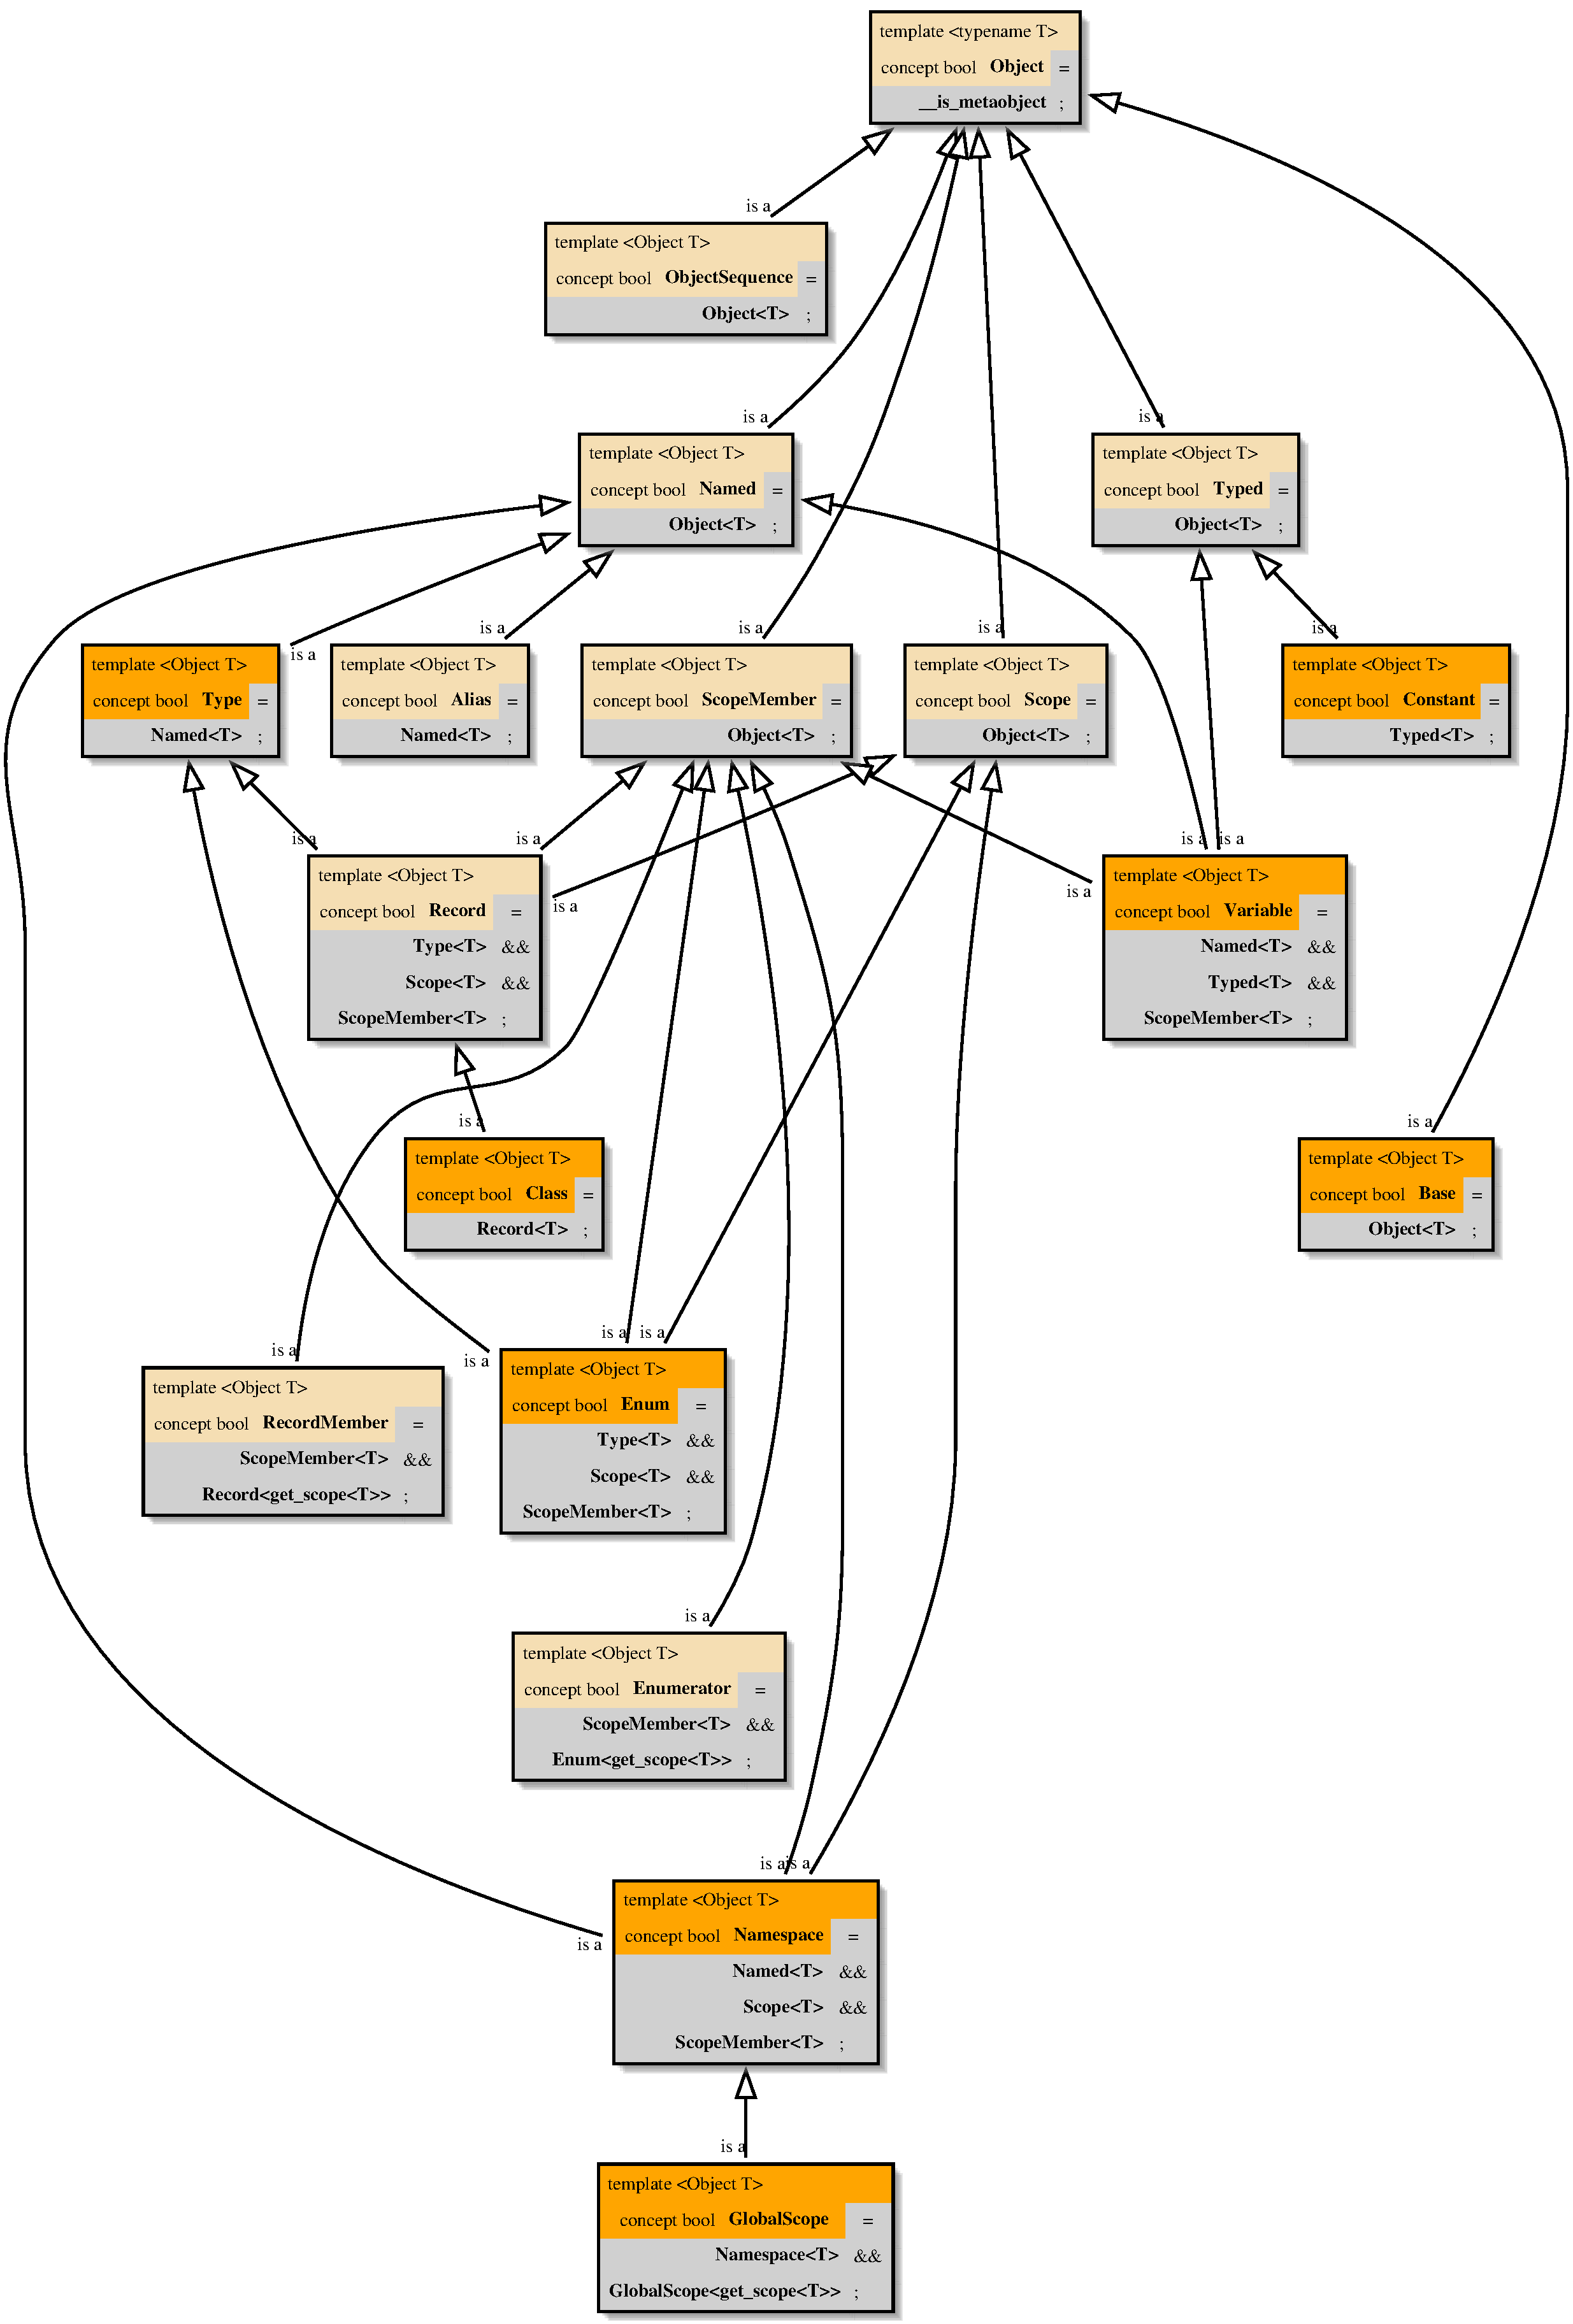
\includegraphics[width=0.81\linewidth]{images/hierarchy.pdf}
\caption{Metaobject concept hierarchy}
\end{figure}

\end{appendices}

\end{document}
